% This must be in the first 5 lines to tell arXiv to use pdfLaTeX, which is strongly recommended.
\pdfoutput=1
% In particular, the hyperref package requires pdfLaTeX in order to break URLs across lines.

\documentclass[11pt]{article}

% Change "review" to "final" to generate the final (sometimes called camera-ready) version.
% Change to "preprint" to generate a non-anonymous version with page numbers.
\usepackage[final]{acl}
%\usepackage{acl}
\usepackage{tikz}
\usetikzlibrary{positioning, arrows.meta}

% Standard package includes
\usepackage{makecell}
\usepackage{times}
\usepackage{latexsym}
\usepackage{booktabs}
\usepackage[ruled,vlined]{algorithm2e}

% For proper rendering and hyphenation of words containing Latin characters (including in bib files)
\usepackage[T1]{fontenc}
% For Vietnamese characters
% \usepackage[T5]{fontenc}
% See https://www.latex-project.org/help/documentation/encguide.pdf for other character sets

% This assumes your files are encoded as UTF8
\usepackage[utf8]{inputenc}

% This is not strictly necessary, and may be commented out,
% but it will improve the layout of the manuscript,
% and will typically save some space.
\usepackage{microtype}

% This is also not strictly necessary, and may be commented out.
% However, it will improve the aesthetics of text in
% the typewriter font.
\usepackage{inconsolata}
%\usepackage[none]{hyphenat}


%Including images in your LaTeX document requires adding
%additional package(s)
\usepackage{graphicx}
\usepackage{adjustbox}
\usepackage{amssymb}
\usepackage{colortbl}
%\usepackage[margin=1in]{geometry}
\usepackage[table]{xcolor}
\usetikzlibrary{positioning}
\usepackage{graphicx}
\usepackage{xcolor}
\usepackage{array}
\usepackage{tikz}
\usepackage{tikz-dependency}
\usepackage[utf8]{inputenc}
\usepackage{amsmath}
\usepackage{caption}
\usepackage{multirow}
\usepackage{pifont}
\usepackage[most]{tcolorbox}
\usepackage{tabularx}
\usepackage{xcolor}
\newcommand{\cmark}{\ding{51}}
\newcommand{\xmark}{\ding{55}}
\definecolor{aspectbg}{RGB}{255,226,194}
\definecolor{harmbg}{RGB}{255,210,214}
\definecolor{categorybg}{RGB}{202,235,247}
\definecolor{rationalebg}{RGB}{255,247,181}
\definecolor{titleblue}{RGB}{20,20,165}

\newcommand{\annlabel}[2]{%
\colorbox{#1}{\strut #2}%
}
\newcommand{\tagbox}[2][gray!15]{%
  \colorbox{#1}{\strut #2}%
}
% If the title and author information does not fit in the area allocated, uncomment the following
%
%\setlength\titlebox{<dim>}
%
% and set <dim> to something 5cm or larger.

% \title{Beyond Surface Toxicity: Benchmarking and Explainable Abusive and Harmful Memes Classification Towards Women Harassment using Neuro-Symbolic Approach}
% \title{Beyond Surface Toxicity: A Neuro-Symbolic Benchmark for Explainable Women-Targeted Abuse and Harassment Detection in Memes}
% \title{SheHarm-Meme: A Neuro-Symbolic Benchmark for Explainable Women-Targeted Harassment and Abuse Detection \\ Beyond Surface Toxicity}
% \title{She is not Harm! Aspect-based Harm Detection using Rule-based Neuro-Symbolic Reasoning towards Women-Targeted Memes}
% \title{SheHarm-CAR: Counterfactual and Aspect-Guided Neuro-Symbolic Reasoning for Women-Targeted Harmful Meme Detection}
\title{SheHarm-CAR: Counterfactual and Rule-Guided Neuro-Symbolic Reasoning for Women-Targeted Harmful Meme Detection}
% \author{
% Lipika Dewangan\textsuperscript{1}, Chandresh Kumar Maurya\textsuperscript{1} \\
% \textsuperscript{1}Indian Institute of Technology Indore, Madhya Pradesh, India 453552 \\
% \texttt{\{phd2101201004, chandresh\}@iiti.ac.in}
% }
% \author{
%   \textbf{Lipika Dewangan\textsuperscript{1}}, 
%   \textbf{Chandresh Kumar Maurya\textsuperscript{1}} \\
%   \textsuperscript{1}Indian Institute of Technology, Indore, Madhya Pradesh, India 453552 \\
%     \texttt{{\{phd2101201004@iiti.ac.in, chandresh@iiti.ac.in\}}
% }}
% \title{CLAOCS-TX: Contrastive Learning with Aspect and Opinion Code-Switching using LLMs to enhance Cross-Lingual Triplet Extraction in Low-Resource Languages}

% Author information can be set in various styles:
% For several authors from the same institution:
% \author{Author 1 \and ... \and Author n \\
%         Address line \\ ... \\ Address line}
% if the names do not fit well on one line use
%         Author 1 \\ {\bf Author 2} \\ ... \\ {\bf Author n} \\
% For authors from different institutions:
% \author{Author 1 \\ Address line \\  ... \\ Address line
%         \And  ... \And
%         Author n \\ Address line \\ ... \\ Address line}
% To start a separate ``row'' of authors use \AND, as in
% \author{Author 1 \\ Address line \\  ... \\ Address line
%         \AND
%         Author 2 \\ Address line \\ ... \\ Address line \And
%         Author 3 \\ Address line \\ ... \\ Address line}


% \author{First Author \\
%   Affiliation / Address line 1 \\
%   Affiliation / Address line 2 \\
%   Affiliation / Address line 3 \\
%   \texttt{email@domain} \\\And
%   Second Author \\
%   Affiliation / Address line 1 \\
%   Affiliation / Address line 2 \\
%   Affiliation / Address line 3 \\
%   \texttt{email@domain} \\}

%\author{
%  \textbf{First Author\textsuperscript{1}},
%  \textbf{Second Author\textsuperscript{1,2}},
%  \textbf{Third T. Author\textsuperscript{1}},
%  \textbf{Fourth Author\textsuperscript{1}},
%\\
%  \textbf{Fifth Author\textsuperscript{1,2}},
%  \textbf{Sixth Author\textsuperscript{1}},
%  \textbf{Seventh Author\textsuperscript{1}},
%  \textbf{Eighth Author \textsuperscript{1,2,3,4}},
%\\
%  \textbf{Ninth Author\textsuperscript{1}},
%  \textbf{Tenth Author\textsuperscript{1}},
%  \textbf{Eleventh E. Author\textsuperscript{1,2,3,4,5}},
%  \textbf{Twelfth Author\textsuperscript{1}},
%\\
%  \textbf{Thirteenth Author\textsuperscript{3}},
%  \textbf{Fourteenth F. Author\textsuperscript{2,4}},
%  \textbf{Fifteenth Author\textsuperscript{1}},
%  \textbf{Sixteenth Author\textsuperscript{1}},
%\\
%  \textbf{Seventeenth S. Author\textsuperscript{4,5}},
%  \textbf{Eighteenth Author\textsuperscript{3,4}},
%  \textbf{Nineteenth N. Author\textsuperscript{2,5}},
%  \textbf{Twentieth Author\textsuperscript{1}}
%\\
%\\
%  \textsuperscript{1}Affiliation 1,
%  \textsuperscript{2}Affiliation 2,
%  \textsuperscript{3}Affiliation 3,
%  \textsuperscript{4}Affiliation 4,
%  \textsuperscript{5}Affiliation 5
%\\
%  \small{
%    \textbf{Correspondence:} \href{mailto:email@domain}{email@domain}
%  }
%}

%\tikzset{out/.style={}}
\begin{document}
\maketitle
\begin{abstract}
Women-targeted harm in memes may be conveyed through sexual
harassment, violence, misogyny, appearance attacks, and character
assassination. Such harm may be explicit or may emerge implicitly
from the interaction between image and text. We introduce
\textbf{SheHarm-Meme}, a multi-task benchmark for explainable
women-targeted harmful meme understanding. It supports four tasks:
women-related target identification, three-way harmfulness
classification, five-way harm-category classification, and
evidence-grounded rationale generation. We further propose
\textbf{SheHarm-CAR}, a counterfactual, target-guided, and
rule-grounded neuro-symbolic framework that identifies the
women-related target, retrieves target-relevant concepts from a
Women-Harm Knowledge Ontology, and contrasts harm-supporting rules
with contextual exception rules. Confidence-gated fusion integrates
multimodal, ontological, and symbolic evidence, while
neural--symbolic consistency and counterfactual learning encourage
predictions and rationales to depend on relevant evidence.
\textsc{SheHarm-CAR} achieves 84.62 Harm-F1, 76.88 Joint-F1,
89.34 BERTScore, and 85.6 counterfactual faithfulness, outperforming
the strongest baseline by 2.04 and 2.59 points in Harm-F1 and
Joint-F1, respectively. These results suggest that target-conditioned
ontology retrieval, contrastive rule reasoning, and counterfactual
learning improve predictive performance and rationale faithfulness.
\end{abstract}
% The benchmark supports joint evaluation of target
% identification, implicit-harm reasoning, harm categorization, and
% faithful explanation generation.
%\end{abstract}
% \begin{abstract}
% Internet memes can convey women-targeted harassment and abuse through
% sexual remarks, violence, misogyny, appearance attacks, character
% assassination, sarcasm, and culturally grounded references. Detecting
% such content is challenging because harmful meaning may be explicit or
% may emerge implicitly from image--text interaction. We introduce
% \textbf{SheHarm-Meme}, a multi-task benchmark for explainable
% women-targeted harmful meme understanding. The benchmark supports four
% tasks: (i) women-targeted aspect-span extraction, (ii) three-way
% harmfulness classification into \textit{Explicit-Harm},
% \textit{Implicit-Harm}, and \textit{Non-Harm}, (iii) fine-grained
% abuse-category classification into \textit{Sexual-Harassment},
% \textit{Violence}, \textit{Misogyny}, \textit{Appearance-Attack}, and
% \textit{Character-Assassination}, and (iv) evidence-grounded rationale
% generation. We further propose \textbf{SheHarm-CAR}, a counterfactual,
% aspect-guided, and rule-grounded neuro-symbolic framework. The model
% first extracts the women-related target, uses the predicted aspect to
% retrieve relevant concepts from a Women-Harm Knowledge Ontology, and
% contrasts harm-supporting rules with contextual exception rules.
% Confidence-gated neural--symbolic fusion integrates multimodal evidence,
% retrieved knowledge, and activated rules for joint prediction. A
% neural--symbolic consistency objective aligns model decisions with
% symbolic evidence, while counterfactual interventions encourage the
% predictions and generated rationales to depend on target-relevant
% multimodal cues. SheHarm-Meme provides a unified testbed for
% target identification, harmfulness detection, abuse categorization,
% implicit-harm reasoning, and faithful explanation generation.
% \end{abstract}


% \begin{figure}[t]
% \centering
% \begin{tcolorbox}[
%     width=\columnwidth,
%     enhanced,
%     colback=white,
%     colframe=titleblue,
%     boxrule=0.8pt,
%     arc=3mm,
%     left=2mm,
%     right=2mm,
%     top=1.5mm,
%     bottom=1.5mm,
%     title={\centering\textbf{Example of SheHarm-Meme Annotation}},
%     colbacktitle=titleblue,
%     coltitle=white,
%     fonttitle=\small,
%     attach boxed title to top center={yshift=-0.5mm},
%     boxed title style={
%         width=0.82\linewidth,
%         sharp corners=south,
%         arc=2mm,
%         boxrule=0pt
%     }
% ]

% \small

% \begin{tcolorbox}[
%     colback=gray!6,
%     colframe=gray!30,
%     boxrule=0.4pt,
%     arc=1.5mm,
%     left=1.5mm,
%     right=1.5mm,
%     top=1mm,
%     bottom=1mm
% ]
% \textbf{OCR Text:}
% \textit{Look at her face; no one would ever choose her for the
% advertisement.}
% \end{tcolorbox}

% \vspace{1mm}

% \renewcommand{\arraystretch}{1.22}
% \begin{tabularx}{\linewidth}{
%     @{}
%     >{\bfseries\raggedright\arraybackslash}p{0.36\linewidth}
%     >{\raggedright\arraybackslash}X
%     @{}
% }

% Women-related aspect &
% \colorbox{aspectbg}{\strut her face}
% \\

% Harmfulness &
% \colorbox{harmbg}{\strut\textit{Explicit-Harm}}
% \\

% Harm category &
% \colorbox{categorybg}{\strut\textit{Appearance-Attack}}
% \\

% \raisebox{-0.2\height}{Rationale} &
% \begin{tcolorbox}[
%     colback=rationalebg,
%     colframe=rationalebg,
%     boxrule=0pt,
%     arc=0.5mm,
%     left=1mm,
%     right=1mm,
%     top=0.5mm,
%     bottom=0.5mm,
%     width=\linewidth
% ]
% The meme attacks the woman's appearance and links it to her
% suitability for advertising.
% \end{tcolorbox}
% \\

% \end{tabularx}
% \end{tcolorbox}

% \caption{Illustrative SheHarm-Meme annotation comprising a
% women-related aspect span, harmfulness label, harm category, and
% evidence-grounded rationale.}
% \label{fig:annotation-example}
% \end{figure}
% \section{Introduction}
% \label{sec:introduction}

% Internet memes have become a prominent form of online communication,
% combining visual content with short textual expressions to convey
% humour, opinions, and social commentary. The same expressive
% flexibility, however, enables memes to circulate harassment, abuse,
% and discriminatory beliefs while appearing humorous or innocuous.
% Women-targeted memes may communicate sexual harassment, threats,
% misogynistic beliefs, appearance-based attacks, and character
% assassination through direct insults or indirect stereotypes,
% innuendo, sarcasm, and culturally grounded references. Their
% harmfulness therefore cannot always be identified from offensive
% words alone, because the intended meaning may emerge from visual
% symbolism, background knowledge, or the interaction between
% individually benign image and text components
% \citep{kiela2020hateful,kumar2022hate,burbi2023mapping,
% lin2023beneath}.
\section{Introduction}
\label{sec:introduction}

Internet memes combine images and short text to communicate humour,
opinions, and social commentary
\citep{hee2025demystifying,chen2025adammeme}. The same format can also
spread women-targeted harassment and discriminatory beliefs while
appearing humorous or harmless
\citep{lin2025explainhm++}. Such memes%
\footnote{\textbf{Content warning:} This paper contains examples and
discussion of women-targeted abusive, violent, misogynistic, and
discriminatory content that some readers may find disturbing.}
may express sexual harassment, violence, misogyny, appearance attacks,
and character assassination through direct insults, stereotypes,
innuendo, sarcasm, or culturally grounded references
\citep{kumari2025memedetoxnet}. Their harmfulness may arise from visual
symbolism, background knowledge, or interactions between individually
benign image and text components
\citep{kiela2020hateful,kumar2022hate,burbi2023mapping,
lin2023beneath}.

%%%intro example
\begin{figure}[t]
\centering
\begin{tcolorbox}[
    width=\linewidth,
    colback=blue!2,
    colframe=blue!60!black,
    coltitle=white,
    colbacktitle=blue!60!black,
    title=\textbf{SheHarm-Meme Annotation Example},
    fonttitle=\small\bfseries,
    boxrule=0.7pt,
    arc=2mm,
    left=1.4mm,
    right=1.4mm,
    top=1mm,
    bottom=1mm
]

\centering

\includegraphics[
    width=\linewidth,
    height=4.1cm,
    keepaspectratio
]{get_back.jpeg}

\vspace{0.8mm}

\begin{tcolorbox}[
    colback=gray!8,
    colframe=gray!35,
    boxrule=0.3pt,
    arc=1mm,
    left=1mm,
    right=1mm,
    top=0.6mm,
    bottom=0.6mm
]
\small
\textbf{OCR Text:}
\textit{Get back in the kitchen!}
\end{tcolorbox}

\vspace{0.8mm}

\small
\begin{tabularx}{\linewidth}{@{}p{0.33\linewidth}X@{}}
\textbf{Women-related Target}
& \tagbox[orange!18]{woman being struck} \\[0.8mm]

\textbf{Harmfulness}
& \tagbox[pink!20]{\textit{Explicit-Harm}} \\[0.8mm]

\textbf{Harm Category}
& \tagbox[cyan!18]{\textit{Violence}} \\[0.8mm]

\textbf{Rationale}
& \tagbox[yellow!25]{%
\parbox[t]{0.96\linewidth}{%
The meme reinforces the stereotype that women belong in the kitchen
while depicting aggression toward a woman.}} \\
\end{tabularx}

\end{tcolorbox}

\caption{SheHarm-Meme annotation for explicit misogyny conveyed
through a gender-role stereotype and supporting visual aggression.}
\label{fig:sheharm_annotation_example}
\end{figure}
%%%
Most harmful-meme studies formulate the task as binary multimodal
classification using feature fusion, cross-modal interaction, or
multimodal pretraining
\citep{kumar2022hate,burbi2023mapping}. More recent methods use large
language or multimodal models to obtain external knowledge, reasoning
traces, and natural-language explanations
\citep{lin2023beneath,lin2025explainhm++,
tzelepi2024exploiting}. Although these approaches improve implicit-harm
detection, a meme-level label does not identify the targeted woman or
women-related entity, the form of harm, or the evidence supporting the
decision. Multimodal misogyny benchmarks provide fine-grained labels
for stereotyping, objectification, shaming, hostility, and violence
\citep{fersini2022semeval,muti2022unibo}, together with explanation
generation for women-targeted memes
\citep{kanwar2025beneath}. However, explicit and implicit harms are
often merged, and generated rationales may remain plausible without
reflecting the evidence actually used by the model
\citep{lin2023beneath,lin2025explainhm++}.

Implicit harm may additionally depend on social, cultural, and
commonsense knowledge absent from the meme itself. Existing methods
therefore incorporate LMM-generated descriptions or external resources
such as ConceptNet and Wikidata
\citep{tzelepi2024exploiting,tripathi2026they}. Retrieved knowledge,
however, may be unrelated to the actual target and does not by itself
provide a transparent reasoning process. Neuro-symbolic learning offers
a complementary direction by combining neural representations with
structured knowledge and interpretable rules
\citep{liu2025neural,wang2025rule}. This is particularly useful for
distinguishing harmful endorsement from quotation, criticism,
awareness, and counter-speech.

We introduce \textbf{SheHarm-Meme}, a multi-task benchmark for
explainable women-targeted harmful meme understanding. It supports four
tasks: \textit{(i)} women-related target identification,
\textit{(ii)} three-way harmfulness classification into
\textit{Explicit-Harm}, \textit{Implicit-Harm}, and
\textit{Non-Harm}, \textit{(iii)} five-way harm-category
classification, and \textit{(iv)} evidence-grounded rationale
generation. Harmful memes receive one of five categories:
\textit{Sexual-Harassment}, \textit{Violence}, \textit{Misogyny},
\textit{Appearance-Attack}, or
\textit{Character-Assassination}; for \textit{Non-Harm} memes, the
category is set to \textit{None} and excluded from category training
and evaluation.

We further propose \textbf{SheHarm-CAR}, a counterfactual,
target-guided, and rule-guided neuro-symbolic framework. It identifies
the women-related target, retrieves target-relevant concepts from a
Women-Harm Knowledge Ontology, contrasts harm-supporting rules with
contextual exception rules, and integrates multimodal, ontological,
and symbolic evidence through confidence-gated fusion.
Neural--symbolic consistency aligns predictions with activated rules,
while counterfactual interventions encourage harmfulness, category,
and rationale outputs to depend on relevant evidence.

Our contributions are threefold:
\begin{itemize}
\setlength{\itemsep}{1pt}
\setlength{\parskip}{0pt}
\setlength{\parsep}{0pt}

\item We introduce \textbf{SheHarm-Meme}, a four-task benchmark with
ontology-linked women-related targets, explicit/implicit/non-harmful
labels, five harm categories, and human-written rationales.

\item We propose \textbf{SheHarm-CAR}, which combines
target-conditioned ontology retrieval with contrastive
harm-supporting and contextual exception rules.

\item We develop confidence-gated neural--symbolic fusion,
consistency regularization, and counterfactual learning, and evaluate
their effects through main-task performance, implicit-harm analysis,
ablations, and rationale-faithfulness measures.
\end{itemize}

% The main contributions of our study are:

% \begin{itemize}
% \setlength{\itemsep}{1pt}
% \setlength{\parskip}{0pt}
% \setlength{\parsep}{0pt}

% \item We introduce \textbf{SheHarm-Meme}, a four-task benchmark with
% women-related aspect spans, explicit/implicit/non-harmful labels,
% five harm categories, and human-written rationales.

% \item We propose \textbf{SheHarm-CAR}, which performs
% target-conditioned ontology retrieval and contrasts harm-supporting
% rules with contextual exception rules.

% \item We develop confidence-gated neural--symbolic fusion,
% consistency regularization, and counterfactual faithfulness learning
% to align predictions, symbolic evidence, and rationales.

% \item We evaluate the framework through task performance,
% implicit-harm analysis, ablations, rule--decision alignment, and
% counterfactual rationale faithfulness.
% \end{itemize}

% Most harmful meme detection studies formulate the problem as binary
% multimodal classification. Early approaches combined visual and
% textual representations through feature fusion, multimodal
% pretraining, or explicit cross-modal interaction
% \citep{kumar2022hate,burbi2023mapping}. More recent methods use
% large language models and large multimodal models to obtain
% contextual knowledge, reasoning traces, competing interpretations,
% or natural-language explanations
% \citep{lin2023beneath,lin2025explainhm++,tzelepi2024exploiting}.
% These advances improve the recognition of implicit harmfulness, but
% a binary decision provides limited information about the precise
% target, the manner in which harm is expressed, and the evidence that
% supports the prediction. Such information is important for
% moderation systems, where a harmfulness label alone does not explain
% who is targeted, what category of abuse is present, or why the
% image--text combination is harmful.

% Research on multimodal misogyny has begun to address this limitation
% through fine-grained classification schemes covering stereotypes,
% objectification, shaming, hostility, and violence
% \citep{fersini2022semeval,muti2022unibo}. Recent work has also
% examined natural-language explanations for misogynistic or
% women-targeted memes \citep{kanwar2025beneath}. Nevertheless,
% several gaps remain. First, explicit and implicit harms are often
% merged into a single harmful class, although implicit memes require
% reasoning over indirect associations, visual cues, humour, and
% cultural context. Second, existing formulations generally predict a
% meme-level label without explicitly identifying the women-related
% expression being targeted. Third, category inventories are often
% specific to a particular dataset or social context and may not
% capture broadly recurring forms of women-targeted abuse. Finally,
% generated explanations can be plausible but unsupported, because
% they are commonly produced after the classification decision without
% verifying whether the model actually relied on the stated evidence
% \citep{lin2023beneath,lin2025explainhm++}.

% Explicit target identification is particularly important for
% women-targeted meme understanding. A meme may mention several people,
% objects, or social roles, while only one expression is associated
% with the harmful implication. Identifying the shortest meaningful
% women-related aspect span enables a model to distinguish the target
% from surrounding context and to condition subsequent categorization
% and explanation on the relevant evidence. It also supports more
% structured evaluation by requiring the model to answer four connected
% questions: who or what is targeted, whether the meme is harmful, what
% form the harm takes, and why the interpretation is justified.

% Accurate interpretation also requires knowledge that may not be
% explicitly stated in the meme. A model may need to associate a
% depicted social role with a gender stereotype, resolve an indirect
% sexual reference, recognize a reputation-based insinuation, or
% determine whether a harmful expression is endorsed, quoted, or
% criticized. Recent methods enrich meme representations with
% LMM-generated descriptions or external resources such as ConceptNet
% and Wikidata
% \citep{tzelepi2024exploiting,tripathi2026they}. Knowledge infusion
% alone, however, does not guarantee that retrieved concepts are
% relevant to the targeted woman-related aspect, nor that the final
% prediction follows a transparent and verifiable reasoning process.

% Neuro-symbolic learning offers a suitable direction by combining the
% representation capacity of neural models with explicit knowledge and
% interpretable rules. A domain ontology can organize relations among
% women-related roles, harmful expressions, stereotypes, contextual
% modifiers, and abuse categories, while symbolic rules can encode
% reusable reasoning patterns. Rule-guided neural models further allow
% symbolic information to influence training and prediction instead of
% serving only as a post-hoc explanation
% \citep{liu2025neural,wang2025rule}. This combination is especially
% relevant to implicit harm, where a reliable decision should be
% supported by a traceable relationship among the targeted aspect,
% multimodal cues, retrieved knowledge, and the applicable harm or
% exception rule.

% We introduce \textbf{SheHarm-Meme}, a multi-task benchmark for
% explainable women-targeted harmful meme understanding. The benchmark
% supports four complementary tasks: \textit{(i)} women-targeted
% aspect-span extraction, \textit{(ii)} three-way harmfulness
% classification into \textit{Explicit-Harm}, \textit{Implicit-Harm},
% and \textit{Non-Harm}, \textit{(iii)} fine-grained abuse-category
% classification, and \textit{(iv)} evidence-grounded rationale
% generation. Harmful memes are assigned one of five categories:
% \textit{Sexual-Harassment}, \textit{Violence}, \textit{Misogyny},
% \textit{Appearance-Attack}, or
% \textit{Character-Assassination}. For \textit{Non-Harm} memes, the
% category is set to \textit{None} and treated as a null value rather
% than an abuse category.

% Along with the benchmark, we propose \textbf{SheHarm-CAR}, a
% counterfactual, aspect-guided, and rule-grounded neuro-symbolic
% framework. The model first obtains cross-modal representations and
% extracts the women-related aspect span. The predicted aspect is then
% used to retrieve target-relevant concepts from a Women-Harm Knowledge
% Ontology. Instead of activating only harm-supporting rules, the
% framework contrasts them with contextual exception rules representing
% criticism, quotation, awareness, counter-speech, and other
% non-harmful interpretations. A confidence gate controls the
% contribution of retrieved knowledge and symbolic reasoning when
% forming the final prediction.

% The framework jointly predicts the harmfulness label, abuse category,
% and textual rationale from multimodal, aspect-specific, ontological,
% and symbolic evidence. A neural--symbolic consistency objective
% encourages agreement between learned predictions and activated rules.
% In addition, counterfactual interventions remove target-relevant or
% irrelevant evidence during training. Removing relevant evidence is
% expected to reduce confidence in the original prediction, whereas
% removing irrelevant evidence should leave the decision stable. This
% design encourages the predicted label, activated rule, and generated
% rationale to rely on the same target-specific multimodal evidence
% rather than on unsupported post-hoc reasoning.

% The main contributions of this work are as follows:

% \begin{itemize}
%     \item We introduce \textbf{SheHarm-Meme}, a multimodal benchmark
%     that distinguishes explicit, implicit, and non-harmful
%     women-targeted memes and provides women-related aspect spans,
%     fine-grained abuse categories, and human-written rationales.

%     \item We formulate women-targeted harmful meme understanding as
%     four joint tasks: aspect-span extraction, harmfulness
%     classification, abuse-category classification, and
%     evidence-grounded rationale generation.

%     \item We propose \textbf{SheHarm-CAR}, an aspect-guided
%     neuro-symbolic framework that performs target-conditioned
%     ontology retrieval and contrasts harm-supporting rules with
%     contextual exception rules.

%     \item We introduce confidence-gated neural--symbolic fusion,
%     consistency regularization, and counterfactual faithfulness
%     learning to align model predictions, symbolic evidence, and
%     generated rationales.

%     \item We evaluate the proposed framework through task-specific
%     performance, implicit-harm analysis, ablation studies,
%     rule--decision alignment, and counterfactual rationale
%     faithfulness.
% \end{itemize}
\paragraph{Research Questions.}
We investigate four research questions:

\noindent\textbf{RQ1:} How accurately can models identify the
women-related target and distinguish between explicit, implicit, and
non-harmful memes?

\noindent\textbf{RQ2:} How effectively can harmful memes be
classified into the five fine-grained harm categories?

\noindent\textbf{RQ3:} Does target-conditioned ontology retrieval and
contrastive rule reasoning improve performance over standard
multimodal models?

\noindent\textbf{RQ4:} Do neural--symbolic consistency and
counterfactual learning improve the faithfulness and informativeness
of generated rationales?
% \paragraph{Research Questions.}
% We investigate the following research questions:

% \noindent\textbf{RQ1:} How accurately can multimodal models extract
% the women-related aspect span from OCR text in the presence of
% image-dependent and implicit context?

% \noindent\textbf{RQ2:} How effectively can models distinguish
% \textit{Explicit-Harm}, \textit{Implicit-Harm}, and
% \textit{Non-Harm}, and classify harmful memes into the five
% fine-grained abuse categories?

% \noindent\textbf{RQ3:} Does aspect-conditioned ontology retrieval
% improve harmfulness and abuse-category prediction compared with
% standard multimodal fusion and non-target-conditioned knowledge
% integration?

% \noindent\textbf{RQ4:} Do contrastive harm and contextual exception
% rules, together with confidence-gated neural--symbolic fusion,
% improve implicit-harm reasoning and decision interpretability?

% \noindent\textbf{RQ5:} To what extent do neural--symbolic consistency
% and counterfactual interventions improve the faithfulness,
% target alignment, and informativeness of generated rationales?

\section{Related Work}
\label{sec:related-work}

\paragraph{Harmful and misogynistic memes.}
The Hateful Memes Challenge established meme harm detection as a
multimodal task requiring joint image--text interpretation
\citep{kiela2020hateful}. Later methods strengthened cross-modal
interaction using CLIP, prompting, and textual inversion
\citep{kumar2022hate,cao2022prompthate,burbi2023mapping}.
MAMI introduced binary and fine-grained misogyny labels, while
subsequent work examined unintended bias and explanation generation
\citep{fersini2022semeval,muti2022unibo,
kumari2024unintended,kanwar2025beneath}. However, these studies
generally operate at the meme level and do not jointly identify the
targeted women-related aspect, distinguish explicit from implicit
harm, predict a fine-grained abuse category, and generate a supporting
rationale. This motivates a unified four-task benchmark that connects
target identification with harmfulness, categorization, and
explanation.

\paragraph{Explainable and knowledge-guided reasoning.}
Recent approaches generate rationales through LLM distillation,
multimodal debate, retrieval augmentation, or multimodal prompting
\citep{lin2023beneath,lin2024explainhm,
lin2025explainhm++,hee2025demystifying}. External and
LMM-generated knowledge has also been used to improve implicit meme
interpretation
\citep{grasso2024kermit,tzelepi2025improving,
garg2025just,tripathi2026they}. Nevertheless, retrieved knowledge may
be unrelated to the actual target, and fluent rationales may not
reflect the evidence responsible for the prediction. Neuro-symbolic
methods offer a complementary direction by combining neural
representations with structured knowledge and rules
\citep{colelough2025neuro,liu2025neural,wang2025rule}.
Motivated by these limitations, \textsc{SheHarm-CAR} uses the
predicted women-related aspect to retrieve ontology knowledge,
contrasts harm-supporting rules with contextual exception rules, and
applies neural--symbolic consistency and counterfactual learning to
align predictions with target-specific evidence.


%%%%
% \section{Methodology}
% \label{sec:methodology}

% We propose \textsc{SheHarm-CAR}, a counterfactual,
% aspect-guided, and rule-grounded neuro-symbolic framework for
% explainable women-targeted harmful meme detection. Given a meme image
% and its OCR text, the model learns a multimodal representation,
% extracts the women-related aspect, retrieves target-relevant ontology
% concepts, contrasts harm-supporting and contextual exception rules,
% and jointly predicts harmfulness, harm category, and a grounded
% rationale. Figure~\ref{fig:sheharm-car-framework} presents the overall
% architecture.
\section{Methodology}
\label{sec:methodology}

We propose \textsc{SheHarm-CAR}, a counterfactual,
target-guided, and rule-grounded neuro-symbolic framework for
explainable women-targeted harmful meme detection. Given a meme image
and its OCR text, the model learns a multimodal representation,
identifies the women-related target, retrieves target-relevant
ontology concepts, contrasts harm-supporting and contextual exception
rules, and jointly predicts harmfulness, harm category, and a grounded
rationale. Figure~\ref{fig:sheharm-car-framework} presents the overall
architecture.


%%%
\begin{figure*}[t]
    \centering
    
\includegraphics[width=\textwidth]{latex/SheHarm-Meme.png}
    \caption{Architecture of \textsc{SheHarm-CAR}. The framework
    combines women-targeted aspect extraction, aspect-conditioned
    ontology retrieval, contrastive symbolic reasoning,
    confidence-gated neural--symbolic fusion, and counterfactual
    faithfulness learning.}
    \label{fig:sheharm-car-framework}
\end{figure*}
%%
\subsection{Task Formulation}
\label{subsec:task_formulation}

SheHarm-Meme supports four tasks: women-related target
identification, three-way harmfulness classification, five-way
harm-category classification, and evidence-grounded rationale
generation. The women-related target is predicted from the fused
image--text representation over a controlled inventory of
ontology-linked target concepts, allowing targets to be expressed
visually, textually, or through both modalities. Related studies have
identified social entities targeted by harmful memes, detected victims
using textual and visual entity cues, and characterized entities as
victims, villains, or heroes
\citep{pramanick2021harmfulmemes,sharma2022disarm,
sharma2023characterizing}. Unlike these broader entity-level settings,
our task focuses specifically on the woman, female role, body-related
reference, relationship, profession, or women-associated group toward
which the meme's meaning is directed.

Let
\begin{equation}
\mathcal{D}
=
\{(I_i,T_i,t_i,y_i,c_i,r_i)\}_{i=1}^{N},
\end{equation}
where $I_i$ and $T_i$ denote the meme image and OCR text,
$t_i$ is the women-related target label, $y_i$ is the harmfulness
label, $c_i$ is the harm category, and $r_i$ is the
evidence-grounded rationale. The model jointly predicts
\begin{equation}
f_{\theta}(I_i,T_i)
\rightarrow
(\hat{t}_i,\hat{y}_i,\hat{c}_i,\hat{r}_i).
\end{equation}

The harmfulness labels are \textit{Explicit-Harm},
\textit{Implicit-Harm}, and \textit{Non-Harm}. Harmful memes receive
one of five categories: \textit{Sexual-Harassment},
\textit{Violence}, \textit{Misogyny}, \textit{Appearance-Attack}, or
\textit{Character-Assassination}. For \textit{Non-Harm} instances,
$c_i=\textit{None}$ and the category loss is masked.
% \subsection{Task Formulation}
% \label{subsec:task_formulation}

% SheHarm-Meme supports four tasks: women-related target
% identification, three-way harmfulness classification, five-way
% harm-category classification, and evidence-grounded rationale
% generation. The women-related target is predicted from the fused image--text
% representation over a controlled inventory of ontology-linked target
% concepts. This formulation accommodates targets expressed visually,
% textually, or through both modalities. Related studies have identified
% social entities targeted by harmful memes, detected individual victims
% using textual and visual entity cues, and characterized whether entities
% are portrayed as victims, villains, or heroes
% \citep{pramanick2021harmfulmemes,sharma2022disarm,
% sharma2023characterizing}. Unlike these broader entity-level settings,
% our task focuses specifically on the woman, female role, body-related
% reference, or women-associated group toward which the meme's meaning is
% directed.

% Let
% \begin{equation}
% \mathcal{D}
% =
% \{(I_i,T_i,t_i,y_i,c_i,r_i)\}_{i=1}^{N},
% \end{equation}
% where $I_i$ and $T_i$ denote the meme image and OCR text,
% $t_i$ is the women-related target label, $y_i$ is the harmfulness
% label, $c_i$ is the harm category, and $r_i$ is the rationale.
% The model jointly predicts
% \begin{equation}
% f_{\theta}(I_i,T_i)
% \rightarrow
% (\hat{t}_i,\hat{y}_i,\hat{c}_i,\hat{r}_i).
% \end{equation}
% The harmfulness labels are \textit{Explicit-Harm},
% \textit{Implicit-Harm}, and \textit{Non-Harm}. Harmful memes receive
% one of five categories: \textit{Sexual-Harassment},
% \textit{Violence}, \textit{Misogyny}, \textit{Appearance-Attack}, or
% \textit{Character-Assassination}. For \textit{Non-Harm} instances,
% $c_i=\textit{None}$ and the category loss is masked.
% \subsection{Task Formulation}
% \label{subsec:task-formulation}

% Let
% \begin{equation}
% \mathcal{D}
% =
% \{(I_i,T_i,a_i,y_i,c_i,r_i)\}_{i=1}^{N},
% \label{eq:dataset}
% \end{equation}
% where $I_i$ and $T_i$ denote the meme image and OCR text, $a_i$ is the
% women-related aspect span, $y_i$ is the harmfulness label, $c_i$ is
% the harm category, and $r_i$ is a human-written rationale. Figure~\ref{fig:sheharm_example} illustrates the four annotation
% components assigned to each meme.

% The model jointly predicts
% \begin{equation}
% f_{\theta}(I_i,T_i)
% \rightarrow
% (\hat{a}_i,\hat{y}_i,\hat{c}_i,\hat{r}_i).
% \label{eq:prediction-function}
% \end{equation}



\subsection{Multimodal and Target Representation}
\label{subsec:multimodal-target}

Pretrained visual and textual encoders produce patch-level and
token-level representations from the meme image and OCR text.
Bidirectional cross-modal attention allows OCR tokens to attend to
visual regions and image patches to attend to textual cues. The pooled
outputs are fused into a global multimodal representation
$\mathbf{z}_i$.

Unlike textual aspect extraction, the women-related target may be
expressed visually, textually, or through their interaction. We
therefore formulate target identification as classification over a
controlled inventory of ontology-linked women-related target concepts.
The target distribution is predicted as

\begin{equation}
\mathbf{p}^{t}_i
=
\operatorname{softmax}
\left(
\mathbf{W}_{t}\mathbf{z}_i+\mathbf{b}_{t}
\right),
\label{eq:target-distribution}
\end{equation}

where each class corresponds to a canonical target concept, such as
\textit{woman passenger}, \textit{female politician},
\textit{woman's face}, or \textit{women as a group}. The target
classifier is supervised using cross-entropy:

\begin{equation}
\mathcal{L}_{\mathrm{tgt}}
=
-\sum_{i=1}^{N}
\log p^{t}_{i,t_i},
\label{eq:target-loss}
\end{equation}

where $t_i$ denotes the gold target label.

To preserve prediction uncertainty and enable differentiable
target-conditioned reasoning, we compute a soft target representation:

\begin{equation}
\widetilde{\mathbf{t}}_i
=
\sum_{m=1}^{M}
p^{t}_{im}\mathbf{e}^{t}_{m},
\label{eq:target-representation}
\end{equation}

where $M$ is the number of target concepts and
$\mathbf{e}^{t}_{m}$ is the embedding of target concept $m$.
Downstream retrieval, rule reasoning, classification, and rationale
generation modules use $\widetilde{\mathbf{t}}_i$ during both training
and inference.
\subsection{Target-Conditioned Ontology Retrieval}
\label{subsec:knowledge-retrieval}

We construct a Women-Harm Knowledge Ontology containing
women-related targets, harmful expressions, harm categories,
contextual exceptions, and multimodal evidence. Each knowledge item
is represented as a triple $\langle h,r,t\rangle$, where $h$, $r$,
and $t$ denote the head entity, relation, and tail entity,
respectively. Table~\ref{tab:ontology_examples} presents representative ontology
relations covering women-related targets, harm cues, contextual
exceptions, and multimodal evidence. The ontology contains 611 concepts, 14 relation types, 1,287 triples,
and 36 soft reasoning rules; the complete inventory is provided in
the appendix.
Table~\ref{tab:ontology-statistics} summarizes the ontology
statistics.

The retrieval query is conditioned on the global meme representation
and the predicted soft target representation:

\begin{equation}
\mathbf{q}^{K}_i
=
\operatorname{LayerNorm}
\left(
\mathbf{W}_{q}
\left(
\mathbf{z}_i
\mathbin{\Vert}
\widetilde{\mathbf{t}}_i
\right)
+
\mathbf{b}_{q}
\right).
\label{eq:retrieval-query}
\end{equation}

The top-$K$ ontology concepts are selected using cosine similarity
between $\mathbf{q}^{K}_i$ and each ontology concept embedding
$\mathbf{k}_u$. The retrieved knowledge representation is

\begin{equation}
\widetilde{\mathbf{k}}_i
=
\sum_{u \in \mathcal{N}_{K}(i)}
\alpha_{iu}\mathbf{k}_u,
\label{eq:retrieved-knowledge}
\end{equation}

where

\begin{equation}
\alpha_{iu}
=
\frac{
\exp(s_{iu}/\tau)
}{
\sum_{v \in \mathcal{N}_{K}(i)}
\exp(s_{iv}/\tau)
},
\label{eq:knowledge-weight}
\end{equation}

$s_{iu}$ is the cosine similarity between the query and concept $u$,
and $\tau$ is a temperature parameter. A contrastive alignment loss
$\mathcal{L}_{\mathrm{align}}$ brings the target-conditioned query
closer to relevant ontology concepts while separating it from sampled
negative concepts. 
\begin{table}[t]
\centering
\small
\setlength{\tabcolsep}{3.5pt}
\renewcommand{\arraystretch}{1.08}
\begin{tabular}{p{0.18\linewidth}p{0.23\linewidth}
                p{0.22\linewidth}p{0.27\linewidth}}
\toprule
\textbf{Type} &
\textbf{Head} &
\textbf{Relation / Tail} &
\textbf{Reasoning Role} \\
\midrule

Target
& woman passenger
& \textit{is-a} Female-Role
& Identifies the women-related target. \\

Target
& her face
& \textit{is-a} Female-Appearance
& Grounds an appearance-related target. \\

Harm cue
& ``too ugly''
& \textit{expresses} Appearance-Attack
& Links appearance ridicule to its category. \\

Harm cue
& ``beat her''
& \textit{expresses} Violence
& Encodes physical-harm evidence. \\

Harm cue
& ``belongs in the kitchen''
& \textit{expresses} Misogyny
& Represents a gender-role stereotype. \\

Context
& harmful statement
& \textit{negated-by} Condemnation
& Reduces harm support under criticism. \\

Context
& harmful phrase
& \textit{quoted-in} Counter-Speech
& Distinguishes quotation from endorsement. \\

Evidence
& Violence
& \textit{supported-by} Visual Injury
& Connects a category to visual evidence. \\

\bottomrule
\end{tabular}
\caption{Representative concepts and relations from the Women-Harm
Knowledge Ontology. Contextual relations encode exceptions that
distinguish harmful endorsement from quotation, criticism, and
counter-speech.}
\label{tab:ontology_examples}
\end{table}
\subsection{Contrastive Symbolic Reasoning}
\label{subsec:contrastive-rules}

\begin{table}[t]
\centering
\small
\setlength{\tabcolsep}{4pt}
\renewcommand{\arraystretch}{1.08}
\begin{tabularx}{\columnwidth}{@{}lX@{}}
\toprule
\textbf{Rule} & \textbf{Description} \\
\midrule

R1 &
IF women-related target AND sexualized remark or objectification
THEN \textit{Sexual-Harassment}. \\

R2 &
IF women-related target AND threat, violent intent, or encouragement
of physical harm THEN \textit{Violence}. \\

R3 &
IF women-related target AND gender-based inferiority, exclusion, or
stereotype THEN \textit{Misogyny}. \\

R4 &
IF women-related target AND ridicule of face, body, clothing, or
physical appearance THEN \textit{Appearance-Attack}. \\

R5 &
IF women-related target AND reputation attack, moral judgement, or
derogatory character allegation THEN
\textit{Character-Assassination}. \\

R6 &
IF a harmful cue directly refers to the identified women-related
target THEN increase \textit{Explicit-Harm} support. \\

R7 &
IF the harmful interpretation requires image--text association,
cultural knowledge, sarcasm, or indirect implication THEN increase
\textit{Implicit-Harm} support. \\

R8 &
IF a harmful expression is quoted or depicted AND explicitly
criticized, condemned, or challenged THEN support
\textit{Non-Harm}. \\

R9 &
IF the meme raises awareness, provides counter-speech, or reports harm
without endorsement THEN support \textit{Non-Harm}. \\

R10 &
IF image, OCR text, retrieved knowledge, and activated rules conflict
THEN reduce the neural--symbolic confidence gate. \\

\bottomrule
\end{tabularx}
\caption{Representative harm-supporting, exception, and
confidence-control rules.}
\label{tab:symbolic-rules}
\end{table}

Table~\ref{tab:symbolic-rules} presents representative soft rules for
harm-category prediction, harmfulness reasoning, contextual exception
handling, and confidence control. The rule inventory contains
harm-supporting rules $\mathcal{R}^{+}$ and contextual exception rules
$\mathcal{R}^{-}$. For example, a women-related target combined with
appearance ridicule supports \textit{Appearance-Attack}, whereas an
otherwise harmful expression that is explicitly condemned supports
\textit{Non-Harm}. The rules contribute graded evidence rather than
hard decisions.

Visual relevance is estimated using the cross-modal attention assigned
to image patches, while target-indicative OCR tokens are identified
from text-to-image attention. High-scoring regions and tokens provide
target-relevant evidence, whereas low-attention regions are used for
irrelevant-evidence interventions.

For rule $r_j$, predicate truth values are estimated from the global
multimodal representation $\mathbf{z}_i$, soft target representation
$\widetilde{\mathbf{t}}_i$, and retrieved knowledge
$\widetilde{\mathbf{k}}_i$. Its activation is computed using a soft
conjunction:

\begin{equation}
\rho_{ij}
=
\prod_{l=1}^{m_j} p_{ijl},
\label{eq:rule-activation}
\end{equation}

where $p_{ijl}$ is the estimated truth value of predicate $l$ in rule
$r_j$. The contrastive symbolic representation is

\begin{equation}
\mathbf{q}^{\Delta}_i
=
\sum_{r_j\in\mathcal{R}^{+}}
\rho_{ij}\mathbf{e}_{r_j}
-
\sum_{r_j\in\mathcal{R}^{-}}
\rho_{ij}\mathbf{e}_{r_j},
\label{eq:contrastive-rule-representation}
\end{equation}

where $\mathbf{e}_{r_j}$ denotes the embedding of rule $r_j$. This
contrastive formulation distinguishes harmful endorsement from
quotation, criticism, awareness, and counter-speech. The complete
ontology and rule inventory are provided in the appendix.

\subsection{Confidence-Gated Prediction and Rationale Generation}
\label{subsec:gated-prediction}

Because retrieved knowledge and symbolic rules may be uncertain, a
confidence gate controls their contribution:

\begin{equation}
\gamma_i
=
\sigma
\left(
\mathbf{w}_{g}^{\top}
\left(
\mathbf{z}_i
\mathbin{\Vert}
\widetilde{\mathbf{t}}_i
\mathbin{\Vert}
\widetilde{\mathbf{k}}_i
\mathbin{\Vert}
\mathbf{q}^{\Delta}_i
\right)
+
b_g
\right).
\label{eq:confidence-gate}
\end{equation}

The ontology and symbolic representations are combined as

\begin{equation}
\mathbf{v}_i
=
\mathbf{W}_{K}\widetilde{\mathbf{k}}_i
+
\mathbf{W}_{R}\mathbf{q}^{\Delta}_i,
\label{eq:fused-symbolic}
\end{equation}

and the final reasoning representation is

\begin{equation}
\mathbf{u}_i
=
\operatorname{LayerNorm}
\left(
\mathbf{z}_i
+
\mathbf{W}_{T}\widetilde{\mathbf{t}}_i
+
\gamma_i\mathbf{v}_i
\right).
\label{eq:final-reasoning-representation}
\end{equation}

Separate prediction heads produce the harmfulness and harm-category
distributions:

\begin{equation}
\mathbf{p}^{y}_i
=
\operatorname{softmax}
\left(
\mathbf{W}_{y}\mathbf{u}_i+\mathbf{b}_{y}
\right),
\qquad
\mathbf{p}^{c}_i
=
\operatorname{softmax}
\left(
\mathbf{W}_{c}\mathbf{u}_i+\mathbf{b}_{c}
\right).
\label{eq:prediction-heads}
\end{equation}

The harmfulness loss is

\begin{equation}
\mathcal{L}_{\mathrm{harm}}
=
-
\sum_{i=1}^{N}
\log p^{y}_{i,y_i}.
\label{eq:harmfulness-loss}
\end{equation}

Because \textit{Non-Harm} memes do not receive a harm category, the
category loss is masked:

\begin{equation}
\mathcal{L}_{\mathrm{cat}}
=
-
\sum_{i=1}^{N}
m_i\log p^{c}_{i,c_i},
\label{eq:category-loss}
\end{equation}

where

\begin{equation}
m_i
=
\begin{cases}
1, & y_i \neq \textit{Non-Harm},\\
0, & y_i = \textit{Non-Harm}.
\end{cases}
\label{eq:category-mask}
\end{equation}

The rationale decoder is conditioned on $\mathbf{u}_i$, the predicted
soft target representation, retrieved knowledge, and activated rules.
It is trained using autoregressive cross-entropy
$\mathcal{L}_{\mathrm{rat}}$ to generate a concise explanation that
identifies the target, relevant multimodal evidence, harmfulness, and
harm category.

\subsection{Consistency and Counterfactual Faithfulness}
\label{subsec:faithfulness}

Activated rules are mapped to symbolic harmfulness and category
distributions, denoted by $\mathbf{s}^{y}_i$ and
$\mathbf{s}^{c}_i$. Their agreement with the neural predictions is
encouraged through

\begin{equation}
\mathcal{L}_{\mathrm{cons}}
=
\sum_{i=1}^{N}
D_{\mathrm{KL}}
\left(
\mathbf{s}^{y}_i
\Vert
\mathbf{p}^{y}_i
\right)
+
\sum_{i=1}^{N}
m_i
D_{\mathrm{KL}}
\left(
\mathbf{s}^{c}_i
\Vert
\mathbf{p}^{c}_i
\right).
\label{eq:consistency-loss}
\end{equation}

The consistency loss is applied only when at least one symbolic rule
exceeds a validation-selected activation threshold, thereby limiting
the influence of uncertain rule evidence.

We further construct evidence-based counterfactuals by suppressing
target-relevant image regions or OCR cues, replacing the predicted
target representation with a null representation, removing the
highest-ranked ontology concept, or deactivating the strongest rule.
Removing relevant evidence should reduce confidence in the original
prediction, whereas perturbing low-relevance evidence should preserve
it:

\begin{equation}
\mathcal{L}_{\mathrm{cf}}
=
\mathcal{L}_{\mathrm{nec}}
+
\lambda_{\mathrm{inv}}
\mathcal{L}_{\mathrm{inv}}.
\label{eq:counterfactual-loss}
\end{equation}

Here, $\mathcal{L}_{\mathrm{nec}}$ encourages a confidence decrease
after relevant-evidence removal, while
$\mathcal{L}_{\mathrm{inv}}$ encourages prediction invariance under
irrelevant-evidence perturbation.
\subsection{Joint Training and Inference}
\label{subsec:joint-training}

The supervised four-task objective is

\begin{equation}
\mathcal{L}_{\mathrm{task}}
=
\mathcal{L}_{\mathrm{tgt}}
+
\lambda_{\mathrm{harm}}
\mathcal{L}_{\mathrm{harm}}
+
\lambda_{\mathrm{cat}}
\mathcal{L}_{\mathrm{cat}}
+
\lambda_{\mathrm{rat}}
\mathcal{L}_{\mathrm{rat}}.
\label{eq:task-objective}
\end{equation}

The complete training objective is

\begin{equation}
\mathcal{L}_{\mathrm{total}}
=
\mathcal{L}_{\mathrm{task}}
+
\lambda_{\mathrm{align}}
\mathcal{L}_{\mathrm{align}}
+
\lambda_{\mathrm{cons}}
\mathcal{L}_{\mathrm{cons}}
+
\lambda_{\mathrm{cf}}
\mathcal{L}_{\mathrm{cf}}.
\label{eq:total-objective}
\end{equation}

The coefficients $\lambda_{\mathrm{harm}}$,
$\lambda_{\mathrm{cat}}$, $\lambda_{\mathrm{rat}}$,
$\lambda_{\mathrm{align}}$, $\lambda_{\mathrm{cons}}$, and
$\lambda_{\mathrm{cf}}$ control the respective loss contributions.

At inference, only the meme image and OCR text are provided. The model
predicts the women-related target, retrieves target-relevant ontology
concepts, activates harm-supporting and contextual exception rules,
and outputs the harmfulness label, harm category, and
evidence-grounded rationale. No gold targets, harmfulness labels, harm
categories, or rationales are used at inference.




% \subsection{Joint Training and Inference}
% \label{subsec:joint-training}

% The complete objective is

% \begin{equation}
% \mathcal{L}_{\mathrm{total}}
% =
% \mathcal{L}_{\mathrm{asp}}
% +
% \lambda_{\mathrm{harm}}\mathcal{L}_{\mathrm{harm}}
% +
% \lambda_{\mathrm{cat}}\mathcal{L}_{\mathrm{cat}}
% +
% \lambda_{\mathrm{rat}}\mathcal{L}_{\mathrm{rat}}
% +
% \lambda_{\mathrm{align}}\mathcal{L}_{\mathrm{align}}
% +
% \lambda_{\mathrm{cons}}\mathcal{L}_{\mathrm{cons}}
% +
% \lambda_{\mathrm{cf}}\mathcal{L}_{\mathrm{cf}}.
% \label{eq:total-objective}
% \end{equation}


% \section{Methodology}
% \label{sec:methodology}

% We propose \textsc{SheHarm-CAR}, a counterfactual,
% aspect-guided, and rule-grounded neuro-symbolic framework for
% explainable women-targeted harmful meme detection. The framework
% jointly performs four tasks: women-targeted aspect-span extraction,
% three-way harmfulness classification, fine-grained abuse-category
% classification, and evidence-grounded rationale generation.
% \begin{figure*}[t]
%     \centering
%     
\includegraphics[width=\textwidth]{latex/SHE-HARM-CAR.png}
%     \caption{Architecture of \textsc{SheHarm-CAR}. The framework performs 
%     women-targeted aspect extraction, aspect-conditioned ontology retrieval, 
%     contrastive symbolic rule reasoning, confidence-gated neural--symbolic 
%     fusion, harmfulness and abuse-category classification, and grounded 
%     rationale generation. Neural--symbolic consistency and counterfactual 
%     objectives encourage faithful predictions.}
%     \label{fig:sheharm-car-framework}
% \end{figure*}
% Given a meme image and its OCR text, the framework first learns a
% joint multimodal representation and extracts the women-related target
% span. The predicted aspect representation is used to retrieve relevant
% concepts from a Women-Harm Knowledge Ontology. Harm-supporting rules
% and contextual exception rules are then activated using the
% multimodal, aspect, and retrieved knowledge representations. Their
% outputs are integrated through confidence-gated neural--symbolic
% fusion. Finally, the model predicts the harmfulness label, abuse
% category, and natural-language rationale. Counterfactual interventions
% encourage these outputs to depend on the same target-specific
% multimodal evidence.
% \subsection{Task Formulation}
% \label{subsec:task-formulation}

% Let the dataset be

% \begin{equation}
% \mathcal{D}
% =
% \left\{
% \left(
% I_i,T_i,a_i,y_i,c_i,r_i
% \right)
% \right\}_{i=1}^{N}.
% \label{eq:dataset}
% \end{equation}

% Here, $I_i$ denotes the meme image, $T_i$ is its OCR-extracted
% text, $a_i$ is the women-related aspect span, $y_i$ is the
% harmfulness label, $c_i$ is the abuse-category label, and $r_i$
% is a human-written rationale.

% The benchmark supports four complementary tasks:
% (i) women-targeted aspect-span extraction,
% (ii) three-way harmfulness classification,
% (iii) fine-grained abuse-category classification, and
% (iv) evidence-grounded rationale generation.

% The harmfulness label space comprises \textit{Explicit-Harm},
% \textit{Implicit-Harm}, and \textit{Non-Harm}. Harmful memes are
% assigned one of five harm categories: \textit{Sexual-Harassment},
% \textit{Violence}, \textit{Misogyny}, \textit{Appearance-Attack},
% or \textit{Character-Assassination}. For \textit{Non-Harm} memes,
% the abuse-category label is set to \textit{None}, which is treated
% as a null value and excluded from abuse-category training and
% evaluation.

% Given an input meme $(I_i,T_i)$, the model jointly predicts

% \begin{equation}
% f_{\theta}(I_i,T_i)
% \rightarrow
% \left(
% \hat{a}_i,\hat{y}_i,\hat{c}_i,\hat{r}_i
% \right).
% \label{eq:prediction-function}
% \end{equation}

% Here, $\hat{a}_i$, $\hat{y}_i$, $\hat{c}_i$, and $\hat{r}_i$
% denote the predicted aspect span, harmfulness label, abuse category,
% and rationale, respectively.
% \subsection{Multimodal Meme Encoding}
% \label{subsec:multimodal-encoding}

% The image and OCR text are first encoded using pretrained visual and
% textual encoders. The visual encoder produces patch-level image
% representations:

% \begin{equation}
% \mathbf{H}^{I}_i
% =
% \operatorname{Enc}_{I}(I_i).
% \label{eq:image-encoding}
% \end{equation}

% The textual encoder produces contextualized OCR-token
% representations:

% \begin{equation}
% \mathbf{H}^{T}_i
% =
% \operatorname{Enc}_{T}(T_i).
% \label{eq:text-encoding}
% \end{equation}

% Here, $\mathbf{H}^{I}_i$ and $\mathbf{H}^{T}_i$ contain visual-patch
% and textual-token representations, respectively. Since meme
% harmfulness may emerge only from image--text interaction, we employ
% bidirectional cross-modal attention:

% \begin{equation}
% \widetilde{\mathbf{H}}^{T}_i
% =
% \operatorname{MHA}
% \left(
% \mathbf{H}^{T}_i,
% \mathbf{H}^{I}_i,
% \mathbf{H}^{I}_i
% \right).
% \label{eq:text-conditioned-visual}
% \end{equation}

% \begin{equation}
% \widetilde{\mathbf{H}}^{I}_i
% =
% \operatorname{MHA}
% \left(
% \mathbf{H}^{I}_i,
% \mathbf{H}^{T}_i,
% \mathbf{H}^{T}_i
% \right).
% \label{eq:visual-conditioned-text}
% \end{equation}

% Here, $\operatorname{MHA}$ denotes multi-head attention. The
% cross-modally conditioned representations are pooled as

% \begin{equation}
% \bar{\mathbf{h}}^{I}_i
% =
% \operatorname{Pool}
% \left(
% \widetilde{\mathbf{H}}^{I}_i
% \right).
% \label{eq:pooled-image}
% \end{equation}

% \begin{equation}
% \bar{\mathbf{h}}^{T}_i
% =
% \operatorname{Pool}
% \left(
% \widetilde{\mathbf{H}}^{T}_i
% \right).
% \label{eq:pooled-text}
% \end{equation}

% The global multimodal representation is

% \begin{equation}
% \mathbf{z}_i
% =
% \operatorname{LayerNorm}
% \left(
% \operatorname{FFN}
% \left(
% \bar{\mathbf{h}}^{I}_i
% \mathbin{\Vert}
% \bar{\mathbf{h}}^{T}_i
% \right)
% \right),
% \label{eq:multimodal-representation}
% \end{equation}

% where $\mathbin{\Vert}$ denotes vector concatenation.
% \subsection{Women-Targeted Aspect-Span Extraction}
% \label{subsec:aspect-extraction}

% The aspect module identifies the shortest meaningful OCR span
% referring to the targeted woman, female role, relationship,
% profession, body attribute, behaviour, or another women-related
% expression. Each OCR token is assigned a BIO tag.

% For the $j$-th token, the aspect-tag distribution is

% \begin{equation}
% \mathbf{p}^{a}_{ij}
% =
% \operatorname{softmax}
% \left(
% \mathbf{W}_{a}
% \widetilde{\mathbf{h}}^{T}_{ij}
% +
% \mathbf{b}_{a}
% \right).
% \label{eq:aspect-tagging}
% \end{equation}

% Here, $\widetilde{\mathbf{h}}^{T}_{ij}$ is the cross-modally
% conditioned representation of the $j$-th OCR token. The
% aspect-extraction loss is

% \begin{equation}
% \mathcal{L}_{\mathrm{asp}}
% =
% -
% \sum_{i=1}^{N}
% \sum_{j=1}^{n_i}
% \log
% p^{a}_{ij,a_{ij}},
% \label{eq:aspect-loss}
% \end{equation}

% where $a_{ij}$ is the gold BIO tag.

% To condition the downstream modules on the predicted aspect, we
% compute the probability that each token belongs to the aspect span:

% \begin{equation}
% u_{ij}
% =
% p^{a}_{ij,\mathrm{B}}
% +
% p^{a}_{ij,\mathrm{I}}.
% \label{eq:aspect-membership}
% \end{equation}

% The normalized aspect weight is

% \begin{equation}
% \beta_{ij}
% =
% \frac{
% u_{ij}
% }{
% \sum_{k=1}^{n_i}u_{ik}+\epsilon
% }.
% \label{eq:aspect-weight}
% \end{equation}

% The resulting soft aspect representation is

% \begin{equation}
% \mathbf{a}_i
% =
% \sum_{j=1}^{n_i}
% \beta_{ij}
% \widetilde{\mathbf{h}}^{T}_{ij}.
% \label{eq:aspect-representation}
% \end{equation}

% During training, the aspect extractor is supervised using gold BIO
% tags. All downstream modules are conditioned on the predicted soft
% aspect representation during both training and inference, preventing
% exposure to gold aspects at inference time.
% \subsection{Women-Harm Knowledge Ontology}
% \label{subsec:women-harm-ontology}

% We construct a task-specific Women-Harm Knowledge Ontology:

% \begin{equation}
% \mathcal{K}
% =
% \left(
% \mathcal{E},
% \mathcal{R},
% \mathcal{F}
% \right),
% \label{eq:ontology}
% \end{equation}

% where $\mathcal{E}$ denotes the ontology concepts, $\mathcal{R}$
% denotes the relations, and $\mathcal{F}$ contains factual triples.

% The ontology represents women-related identities and social roles,
% gender stereotypes, sexual harassment, violent actions, appearance
% attacks, character-assassination cues, misogynistic beliefs, and
% contextual modifiers. The contextual concepts include quotation,
% criticism, awareness, counter-speech, negation, reclamation, and
% humour.

% Each ontology fact is represented as

% \begin{equation}
% (h,r,t)
% \in
% \mathcal{F},
% \label{eq:ontology-triple}
% \end{equation}

% where $h$ and $t$ are concepts and $r$ is their relation. Example
% facts include

% \begin{equation}
% \left(
% \textit{sexual-comment},
% \textit{indicates},
% \textit{Sexual-Harassment}
% \right).
% \end{equation}

% \begin{equation}
% \left(
% \textit{violent-threat},
% \textit{indicates},
% \textit{Violence}
% \right).
% \end{equation}

% \begin{equation}
% \left(
% \textit{appearance-ridicule},
% \textit{indicates},
% \textit{Appearance-Attack}
% \right).
% \end{equation}

% \begin{equation}
% \left(
% \textit{reputation-attack},
% \textit{indicates},
% \textit{Character-Assassination}
% \right).
% \end{equation}

% \begin{equation}
% \left(
% \textit{criticism-of-misogyny},
% \textit{supports},
% \textit{Non-Harm}
% \right).
% \end{equation}

% The ontology is initialized using the annotation taxonomy and relevant
% domain literature. Its concepts, relations, and category mappings are
% reviewed to remove ambiguous, redundant, or unsupported entries.
% \subsection{Women-Harm Knowledge Ontology}
% \label{subsec:women-harm-ontology}

% We construct a task-specific Women-Harm Knowledge Ontology
% $\mathcal{K}=(\mathcal{E},\mathcal{R},\mathcal{F})$, where
% $\mathcal{E}$ denotes ontology concepts, $\mathcal{R}$ denotes
% relations, and $\mathcal{F}$ contains factual triples of the form
% $(h,r,t)$. Here, $h$ and $t$ are concepts and $r$ is their relation.

% The ontology represents women-related identities and social roles,
% gender stereotypes, sexual harassment, violent actions, appearance
% attacks, character-assassination cues, misogynistic beliefs, and
% contextual modifiers such as quotation, criticism, awareness,
% counter-speech, negation, reclamation, and humour.
% Table~\ref{tab:ontology-facts} presents representative ontology facts.

% \begin{table}[t]
% \centering
% \small
% \setlength{\tabcolsep}{3.5pt}
% \renewcommand{\arraystretch}{1.05}
% \begin{tabularx}{\columnwidth}{@{}lll@{}}
% \toprule
% \textbf{Head} & \textbf{Relation} & \textbf{Tail} \\
% \midrule
% \textit{sexual-comment}
% & \textit{indicates}
% & \textit{Sexual-Harassment} \\

% \textit{violent-threat}
% & \textit{indicates}
% & \textit{Violence} \\

% \textit{appearance-ridicule}
% & \textit{indicates}
% & \textit{Appearance-Attack} \\

% \textit{reputation-attack}
% & \textit{indicates}
% & \textit{Character-Assassination} \\

% \textit{criticism-of-misogyny}
% & \textit{supports}
% & \textit{Non-Harm} \\
% \bottomrule
% \end{tabularx}
% \caption{Representative facts from the Women-Harm Knowledge Ontology.}
% \label{tab:ontology-facts}
% \end{table}

% The ontology is initialized from the annotation taxonomy and relevant
% domain literature. Its concepts, relations, and category mappings are
% reviewed to remove ambiguous, redundant, or unsupported entries.
% \subsection{Aspect-Conditioned Knowledge Retrieval}
% \label{subsec:knowledge-retrieval}

% The model retrieves ontology concepts that are relevant to both the
% complete meme and the predicted women-related aspect. The retrieval
% query is

% \begin{equation}
% \mathbf{q}^{K}_i
% =
% \operatorname{LayerNorm}
% \left(
% \mathbf{W}_{q}
% \left(
% \mathbf{z}_i
% \mathbin{\Vert}
% \mathbf{a}_i
% \right)
% +
% \mathbf{b}_{q}
% \right).
% \label{eq:retrieval-query}
% \end{equation}

% Let $\mathbf{k}_u$ denote the embedding of ontology concept $u$.
% Its relevance score is calculated using cosine similarity:

% \begin{equation}
% s_{iu}
% =
% \frac{
% \left(
% \mathbf{W}_{m}\mathbf{q}^{K}_i
% \right)^{\top}
% \left(
% \mathbf{W}_{k}\mathbf{k}_u
% \right)
% }{
% \left\|
% \mathbf{W}_{m}\mathbf{q}^{K}_i
% \right\|_{2}
% \left\|
% \mathbf{W}_{k}\mathbf{k}_u
% \right\|_{2}
% }.
% \label{eq:knowledge-score}
% \end{equation}

% Only the top-$K$ concepts are retained:

% \begin{equation}
% \mathcal{N}_{K}(i)
% =
% \operatorname{TopK}_{u\in\mathcal{E}}
% \left(
% s_{iu}
% \right).
% \label{eq:top-k-retrieval}
% \end{equation}

% The normalized relevance weight of concept $u$ is

% \begin{equation}
% \alpha_{iu}
% =
% \frac{
% \exp
% \left(
% s_{iu}/\tau
% \right)
% }{
% \sum_{v\in\mathcal{N}_{K}(i)}
% \exp
% \left(
% s_{iv}/\tau
% \right)
% },
% \label{eq:knowledge-weight}
% \end{equation}

% where $\tau$ is a temperature parameter. The retrieved knowledge
% representation is

% \begin{equation}
% \widetilde{\mathbf{k}}_i
% =
% \sum_{u\in\mathcal{N}_{K}(i)}
% \alpha_{iu}\mathbf{k}_u.
% \label{eq:retrieved-knowledge}
% \end{equation}

% We align the retrieval query with its relevant ontology concept using
% a contrastive objective:

% \begin{equation}
% \mathcal{L}_{\mathrm{align}}
% =
% -
% \sum_{i=1}^{N}
% \log
% \frac{
% \exp
% \left(
% \operatorname{sim}
% \left(
% \mathbf{q}^{K}_i,
% \mathbf{k}^{+}_i
% \right)
% /\tau
% \right)
% }{
% \sum_{u\in\mathcal{B}_i}
% \exp
% \left(
% \operatorname{sim}
% \left(
% \mathbf{q}^{K}_i,
% \mathbf{k}_u
% \right)
% /\tau
% \right)
% }.
% \label{eq:alignment-loss}
% \end{equation}

% Here, $\mathbf{k}^{+}_i$ is a relevant ontology concept and
% $\mathcal{B}_i$ contains the positive concept together with sampled
% negative concepts.
% \subsection{Contrastive Symbolic Rule Reasoning}
% \label{subsec:contrastive-rules}

% We define two complementary rule sets:

% \begin{equation}
% \mathcal{R}
% =
% \mathcal{R}^{+}
% \cup
% \mathcal{R}^{-},
% \label{eq:rule-sets}
% \end{equation}

% where $\mathcal{R}^{+}$ contains harm-supporting rules and
% $\mathcal{R}^{-}$ contains contextual exception rules that support
% a non-harmful interpretation.

% A rule $r_j$ is expressed as

% \begin{equation}
% r_j:
% b_{j1}
% \wedge
% b_{j2}
% \wedge
% \cdots
% \wedge
% b_{jm_j}
% \Rightarrow
% q_j,
% \label{eq:rule-definition}
% \end{equation}

% where $b_{jl}$ denotes a body predicate and $q_j$ denotes the
% conclusion.
% The rule inventory contains harm-supporting rules, contextual
% exception rules, and confidence-control rules. Rather than imposing
% hard logical decisions, each rule is assigned a differentiable
% activation score and contributes soft evidence to the final
% prediction. Table~\ref{tab:symbolic-rules} presents representative
% rules used for harm-category prediction, harmfulness reasoning,
% contextual exception handling, and confidence control.
% Representative harm-supporting rules include

% \begin{equation}
% \textit{Targets-Woman}(x)
% \wedge
% \textit{Sexualizes}(x)
% \Rightarrow
% \textit{Sexual-Harassment}(x).
% \label{eq:sexual-rule}
% \end{equation}

% \begin{equation}
% \textit{Targets-Woman}(x)
% \wedge
% \textit{Expresses-Violence}(x)
% \Rightarrow
% \textit{Violence}(x).
% \label{eq:violence-rule}
% \end{equation}

% \begin{equation}
% \textit{Targets-Woman}(x)
% \wedge
% \textit{Invokes-Gender-Superiority}(x)
% \Rightarrow
% \textit{Misogyny}(x).
% \label{eq:misogyny-rule}
% \end{equation}

% \begin{equation}
% \textit{Targets-Woman}(x)
% \wedge
% \textit{Attacks-Appearance}(x)
% \Rightarrow
% \textit{Appearance-Attack}(x).
% \label{eq:appearance-rule}
% \end{equation}

% \begin{equation}
% \textit{Targets-Woman}(x)
% \wedge
% \textit{Attacks-Character}(x)
% \Rightarrow
% \textit{Character-Assassination}(x).
% \label{eq:character-rule}
% \end{equation}

% Contextual exception rules distinguish harmful endorsement from
% quotation, criticism, awareness, or counter-speech:

% \begin{equation}
% \textit{Mentions-Misogyny}(x)
% \wedge
% \textit{Condemns-Misogyny}(x)
% \Rightarrow
% \textit{Non-Harm}(x).
% \label{eq:condemnation-rule}
% \end{equation}

% \begin{equation}
% \textit{Depicts-Harm}(x)
% \wedge
% \textit{Raises-Awareness}(x)
% \Rightarrow
% \textit{Non-Harm}(x).
% \label{eq:awareness-rule}
% \end{equation}

% For every body predicate, the model estimates a soft truth value:

% \begin{equation}
% p_{ijl}
% =
% \sigma
% \left(
% \mathbf{w}_{jl}^{\top}
% \left(
% \mathbf{z}_i
% \mathbin{\Vert}
% \mathbf{a}_i
% \mathbin{\Vert}
% \widetilde{\mathbf{k}}_i
% \right)
% +
% b_{jl}
% \right).
% \label{eq:predicate-score}
% \end{equation}

% The activation of rule $r_j$ is computed through a differentiable
% soft conjunction:

% \begin{equation}
% \rho_{ij}
% =
% \prod_{l=1}^{m_j}
% p_{ijl}.
% \label{eq:rule-activation}
% \end{equation}

% The harm-supporting rule representation is

% \begin{equation}
% \mathbf{q}^{+}_i
% =
% \sum_{r_j\in\mathcal{R}^{+}}
% \rho_{ij}\mathbf{e}_{r_j}.
% \label{eq:harm-rule-representation}
% \end{equation}

% The exception-rule representation is

% \begin{equation}
% \mathbf{q}^{-}_i
% =
% \sum_{r_j\in\mathcal{R}^{-}}
% \rho_{ij}\mathbf{e}_{r_j}.
% \label{eq:exception-rule-representation}
% \end{equation}

% Here, $\mathbf{e}_{r_j}$ is the learned embedding of rule $r_j$.
% The contrastive symbolic representation is

% \begin{equation}
% \mathbf{q}^{\Delta}_i
% =
% \mathbf{q}^{+}_i
% -
% \mathbf{q}^{-}_i.
% \label{eq:contrastive-rule-representation}
% \end{equation}

% This formulation compares harmful and contextually benign
% interpretations rather than treating every potentially harmful
% expression as sufficient evidence of abuse.
% \subsection{Contrastive Symbolic Rule Reasoning}
% \label{subsec:contrastive-rules}

% We define two complementary rule sets:

% \begin{equation}
% \mathcal{R}
% =
% \mathcal{R}^{+}
% \cup
% \mathcal{R}^{-},
% \label{eq:rule-sets}
% \end{equation}

% where $\mathcal{R}^{+}$ contains harm-supporting rules and
% $\mathcal{R}^{-}$ contains contextual exception rules supporting
% non-harmful interpretations.

% A rule $r_j$ is expressed as

% \begin{equation}
% r_j:
% b_{j1}
% \wedge
% b_{j2}
% \wedge
% \cdots
% \wedge
% b_{jm_j}
% \Rightarrow
% q_j,
% \label{eq:rule-definition}
% \end{equation}

% where $b_{jl}$ denotes a body predicate and $q_j$ denotes the
% conclusion.

% The rule inventory contains harm-supporting rules, contextual
% exception rules, and confidence-control rules. Rather than imposing
% hard logical decisions, each rule is assigned a differentiable
% activation score and contributes soft evidence to the final
% prediction. Table~\ref{tab:symbolic-rules} presents representative
% rules used for harm-category prediction, harmfulness reasoning,
% contextual exception handling, and confidence control.

% % Insert Table~\ref{tab:symbolic-rules} here.

% For each body predicate, the model estimates a soft truth value from
% the multimodal representation, predicted aspect, and retrieved
% ontology knowledge:

% \begin{equation}
% p_{ijl}
% =
% \sigma
% \left(
% \mathbf{w}_{jl}^{\top}
% \left(
% \mathbf{z}_i
% \mathbin{\Vert}
% \mathbf{a}_i
% \mathbin{\Vert}
% \widetilde{\mathbf{k}}_i
% \right)
% +
% b_{jl}
% \right).
% \label{eq:predicate-score}
% \end{equation}
% \subsection{Confidence-Gated Neural--Symbolic Fusion}
% \label{subsec:gated-fusion}

% Ontology retrieval and symbolic rules may occasionally provide
% uncertain or weakly relevant information. We therefore estimate a
% confidence gate:

% \begin{equation}
% g_i
% =
% \sigma
% \left(
% \mathbf{w}_{g}^{\top}
% \left(
% \mathbf{z}_i
% \mathbin{\Vert}
% \mathbf{a}_i
% \mathbin{\Vert}
% \widetilde{\mathbf{k}}_i
% \mathbin{\Vert}
% \mathbf{q}^{\Delta}_i
% \right)
% +
% b_g
% \right).
% \label{eq:confidence-gate}
% \end{equation}

% The retrieved knowledge and symbolic-rule representations are first
% projected into the multimodal feature space:

% \begin{equation}
% \mathbf{v}^{K}_i
% =
% \mathbf{W}_{K}
% \widetilde{\mathbf{k}}_i.
% \label{eq:knowledge-projection}
% \end{equation}

% \begin{equation}
% \mathbf{v}^{R}_i
% =
% \mathbf{W}_{R}
% \mathbf{q}^{\Delta}_i.
% \label{eq:rule-projection}
% \end{equation}

% The final reasoning representation is

% \begin{equation}
% \mathbf{u}_i
% =
% \operatorname{LayerNorm}
% \left(
% \mathbf{z}_i
% +
% \mathbf{W}_{A}\mathbf{a}_i
% +
% g_i
% \left(
% \mathbf{v}^{K}_i
% +
% \mathbf{v}^{R}_i
% \right)
% \right).
% \label{eq:final-reasoning-representation}
% \end{equation}

% A high gate value allows ontology knowledge and symbolic rules to
% strongly influence the decision, whereas a low value causes the model
% to rely primarily on the multimodal evidence.
% \subsection{Harmfulness and Abuse-Category Prediction}
% \label{subsec:classification}

% The harmfulness distribution is

% \begin{equation}
% \mathbf{p}^{y}_i
% =
% \operatorname{softmax}
% \left(
% \mathbf{W}_{y}\mathbf{u}_i
% +
% \mathbf{b}_{y}
% \right).
% \label{eq:harm-prediction}
% \end{equation}

% The harmfulness-classification loss is

% \begin{equation}
% \mathcal{L}_{\mathrm{harm}}
% =
% -
% \sum_{i=1}^{N}
% \log
% p^{y}_{i,y_i}.
% \label{eq:harm-loss}
% \end{equation}

% The abuse-category distribution is computed over the five harmful
% categories:

% \begin{equation}
% \mathbf{p}^{c}_i
% =
% \operatorname{softmax}
% \left(
% \mathbf{W}_{c}\mathbf{u}_i
% +
% \mathbf{b}_{c}
% \right).
% \label{eq:category-prediction}
% \end{equation}

% The category mask is

% \begin{equation}
% m_i
% =
% \begin{cases}
% 1, & y_i \neq \textit{Non-Harm},\\
% 0, & y_i = \textit{Non-Harm}.
% \end{cases}
% \label{eq:category-mask}
% \end{equation}

% The abuse-category loss is

% \begin{equation}
% \mathcal{L}_{\mathrm{cat}}
% =
% -
% \sum_{i=1}^{N}
% m_i
% \log
% p^{c}_{i,c_i}.
% \label{eq:category-loss}
% \end{equation}

% Thus, \textit{None} is retained only as a null annotation for
% \textit{Non-Harm} instances and is not included in the category
% classifier or category-level evaluation.
% \subsection{Evidence- and Rule-Grounded Rationale Generation}
% \label{subsec:rationale-generation}

% The rationale decoder is conditioned on the final reasoning
% representation, predicted aspect, retrieved ontology knowledge, and
% contrastive rule evidence.

% The decoder context is

% \begin{equation}
% \mathbf{d}_i
% =
% \mathbf{W}_{d}
% \left(
% \mathbf{u}_i
% \mathbin{\Vert}
% \mathbf{a}_i
% \mathbin{\Vert}
% \widetilde{\mathbf{k}}_i
% \mathbin{\Vert}
% \mathbf{q}^{\Delta}_i
% \right)
% +
% \mathbf{b}_{d}.
% \label{eq:decoder-context}
% \end{equation}

% The rationale probability is

% \begin{equation}
% p_{\theta}(r_i)
% =
% \prod_{t=1}^{|r_i|}
% p_{\theta}
% \left(
% r_{i,t}
% \mid
% r_{i,<t},
% \mathbf{d}_i
% \right).
% \label{eq:rationale-probability}
% \end{equation}

% The rationale-generation loss is

% \begin{equation}
% \mathcal{L}_{\mathrm{rat}}
% =
% -
% \sum_{i=1}^{N}
% \sum_{t=1}^{|r_i|}
% \log
% p_{\theta}
% \left(
% r_{i,t}
% \mid
% r_{i,<t},
% \mathbf{d}_i
% \right).
% \label{eq:rationale-loss}
% \end{equation}

% The decoder is encouraged to mention the women-related target,
% identify the relevant image--text evidence, and explain the predicted
% harmfulness and abuse category. For non-harmful memes, the rationale
% describes why the content does not endorse or communicate
% women-targeted harm.
% \subsection{Neural--Symbolic Consistency}
% \label{subsec:neural-symbolic-consistency}

% The activated rules are mapped to auxiliary distributions over
% harmfulness labels and abuse categories.

% The symbolic harmfulness distribution is

% \begin{equation}
% \mathbf{s}^{y}_i
% =
% \operatorname{softmax}
% \left(
% \sum_{j=1}^{|\mathcal{R}|}
% \rho_{ij}
% \mathbf{m}^{y}_{j}
% \right).
% \label{eq:symbolic-harm-distribution}
% \end{equation}

% The symbolic category distribution is

% \begin{equation}
% \mathbf{s}^{c}_i
% =
% \operatorname{softmax}
% \left(
% \sum_{j=1}^{|\mathcal{R}|}
% \rho_{ij}
% \mathbf{m}^{c}_{j}
% \right).
% \label{eq:symbolic-category-distribution}
% \end{equation}

% Here, $\mathbf{m}^{y}_{j}$ and $\mathbf{m}^{c}_{j}$ encode the
% harmfulness label and abuse category supported by rule $r_j$.

% The consistency objective is

% \begin{equation}
% \mathcal{L}_{\mathrm{cons}}
% =
% \sum_{i=1}^{N}
% D_{\mathrm{KL}}
% \left(
% \mathbf{s}^{y}_i
% \Vert
% \mathbf{p}^{y}_i
% \right)
% +
% \sum_{i=1}^{N}
% m_i
% D_{\mathrm{KL}}
% \left(
% \mathbf{s}^{c}_i
% \Vert
% \mathbf{p}^{c}_i
% \right).
% \label{eq:consistency-loss}
% \end{equation}

% The loss is applied only when at least one rule activation exceeds a
% validation-selected threshold, preventing uncertain symbolic evidence
% from dominating reliable multimodal predictions.
% \subsection{Counterfactual Faithfulness Learning}
% \label{subsec:counterfactual-learning}

% Plausible rationales are not necessarily faithful to the evidence
% used by a model. We therefore create counterfactual variants that
% remove either target-relevant or irrelevant evidence.

% For an original meme $M_i=(I_i,T_i)$, the evidence-masked
% counterfactual $\widetilde{M}^{e}_i$ is produced by one intervention:
% masking the predicted aspect span, suppressing the most relevant
% visual region, removing the highest-ranked ontology concept, or
% deactivating the highest-scoring symbolic rule.

% Removing relevant evidence should reduce confidence in the gold
% harmfulness label. The necessity loss is

% \begin{equation}
% \mathcal{L}_{\mathrm{nec}}
% =
% \sum_{i=1}^{N}
% \max
% \left(
% 0,
% \gamma
% -
% p_{\theta}
% \left(
% y_i\mid M_i
% \right)
% +
% p_{\theta}
% \left(
% y_i\mid\widetilde{M}^{e}_i
% \right)
% \right).
% \label{eq:necessity-loss}
% \end{equation}

% Here, $\gamma$ is a confidence margin. A neutral counterfactual
% $\widetilde{M}^{n}_i$ is generated by masking low-relevance content.
% The prediction should remain stable under this intervention:

% \begin{equation}
% \mathcal{L}_{\mathrm{inv}}
% =
% \sum_{i=1}^{N}
% D_{\mathrm{KL}}
% \left(
% p_{\theta}
% \left(
% y\mid M_i
% \right)
% \Vert
% p_{\theta}
% \left(
% y\mid\widetilde{M}^{n}_i
% \right)
% \right).
% \label{eq:invariance-loss}
% \end{equation}

% The counterfactual objective is

% \begin{equation}
% \mathcal{L}_{\mathrm{cf}}
% =
% \mathcal{L}_{\mathrm{nec}}
% +
% \lambda_{\mathrm{inv}}
% \mathcal{L}_{\mathrm{inv}}.
% \label{eq:counterfactual-loss}
% \end{equation}

% This objective encourages necessity and invariance: removing
% target-relevant evidence should weaken the prediction, whereas
% removing irrelevant evidence should not substantially change it.


% We describe our proposed approach in this section. As illustrated in Figure~\ref{fig:framework}, the proposed framework consists of three components: (i) LLM-based pseudo triplet generation using aspect- and opinion-aware code-switched prompting, (ii) a student ASTE model trained with English supervision and filtered pseudo triplets, and (iii) triplet-aware contrastive distillation for structured cross-lingual semantic alignment. The LLM plays a dual role as a pseudo-label generator and a semantic teacher during training, while inference relies solely on the student model.  We provide the full step-by-step training and pseudo-label generation algorithm and the prompt template in Appendix \ref{sec:appendix}.




% \subsection{Implementation Details}
% The student ASTE model is based on XLM-R-large ($d=1024$) \citep{conneau2020unsupervised}. Aspect and opinion spans are predicted using independent BIOES taggers with constrained decoding, followed by biaffine scorers for aspect--opinion pairing and sentiment classification. Span representations are obtained via mean pooling over token embeddings. We adopt LLaMA-3-8B-Instruct\footnote{\url{https://huggingface.co/meta-llama/Meta-Llama-3-8B-Instruct}} as a frozen LLM, used only during training for pseudo-label generation and semantic supervision. Generation uses temperature $0.7$, top-$p$ $0.9$, with $K=5$ samples per variant, and triplet embeddings are extracted from the final LLM layer via mean pooling. For each target sentence, up to four variants are constructed (original, aspect-switched, opinion-switched, and joint aspect-opinion-switched). Candidate spans are obtained using high-recall heuristics and low-threshold student predictions, translated into English, and used only for LLM prompting. Pseudo triplets are retained if they appear in at least two samples across two variants and align with contiguous spans in the original sentence, and are weighted by agreement frequency during training. Triplet-aware contrastive distillation is implemented using an InfoNCE objective with 256-dimensional projections and temperature $0.1$, treating other triplets in the mini-batch as negatives. The student is trained on English data for 10 epochs, followed by two rounds of pseudo labeling and retraining with 5 epochs per round. We use the AdamW optimizer with a learning rate of $2\times10^{-5}$, weight decay of $0.01$, batch size $16$, and loss weights $\lambda_1=1.0$ and $\lambda_2=0.5$; a sensitivity analysis of these settings is provided in Table~\ref{tab:hyperparam_sensitivity} in Appendix~\ref{sec:appendix}. All experiments are conducted on a single NVIDIA A100 GPU, with the LLM loaded in 8-bit precision and triplet embeddings cached. We use a single teacher LLM in order to keep the training setup controlled and computationally tractable while isolating the effect of the proposed pseudo-labeling and triplet-aware distillation framework. The proposed method does not depend on model-specific logits or internal states; rather, the LLM is used as a generic pseudo-label generator and semantic teacher through textual outputs and triplet representations. We report detailed training settings only for the proposed framework and for baselines that were re-run in our experimental setup. Results cited directly from prior work are reported under their original published settings and are included as reference comparisons.


% \begin{table}[t]
% \centering
% \small
% \setlength{\tabcolsep}{4pt}
% \caption{Dataset statistics used in our experiments.
% \#s and \#a denote the number of sentences and aspect terms, respectively.
% We follow the data splits provided by \citep{zhang2021cross} for fair comparison.}
% \label{tab:dataset_statistics}
% \begin{tabular}{lcc|cc|cc}
% \toprule
% \multirow{2}{*}{\textbf{Language}} &
% \multicolumn{2}{c|}{\textbf{Train}} &
% \multicolumn{2}{c|}{\textbf{Dev}} &
% \multicolumn{2}{c}{\textbf{Test}} \\
% \cmidrule(lr){2-3} \cmidrule(lr){4-5} \cmidrule(lr){6-7}
%  & \#s & \#a & \#s & \#a & \#s & \#a \\
% \midrule
% English (EN) 
%  & 1600 & 1377 & 400 & 365 & 676 & 612 \\
% Spanish (ES) 
%  & 1656 & 1500 & 414 & 353 & 881 & 713 \\
% French (FR) 
%  & 1332 & 1294 & 322 & 345 & 668 & 649 \\
% Dutch (NL) 
%  & 1378 & 956  & 344 & 274 & 575 & 373 \\
% Russian (RU) 
%  & 2924 & 2439 & 731 & 629 & 1209 & 945 \\
% Turkish (TR) 
%  & 986  & 1083 & 246 & 271 & 144 & 148 \\
% \bottomrule
% \end{tabular}
% \end{table}
% \begin{table*}[t]
% \centering
% \small
% \setlength{\tabcolsep}{4pt}
% \caption{Dataset statistics for cross-lingual ASTE.
% \#s, \#a, and \#o denote the number of sentences, aspect terms, and opinion terms, respectively.
% For zero-shot cross-lingual evaluation, training and validation sets are not available for target languages and are marked as ``--''.}
% \label{tab:dataset_statistics}
% \begin{tabular}{lccc|ccc|ccc}
% \toprule
% \multirow{2}{*}{\textbf{Language}} &
% \multicolumn{3}{c|}{\textbf{Train}} &
% \multicolumn{3}{c|}{\textbf{Validation}} &
% \multicolumn{3}{c}{\textbf{Test}} \\
% \cmidrule(lr){2-4} \cmidrule(lr){5-7} \cmidrule(lr){8-10}
%  & \#s & \#a & \#o & \#s & \#a & \#o & \#s & \#a & \#o \\
% \midrule
% English (EN) 
%  & 2000 & 3693 & 3399 
%  & 676 & 1134 & 1008 
%  & 676 & 1134 & 1008 \\
% \midrule
% French (FR) 
%  & 1332 & 1294 & -- 
%  & 322 & 345 & -- 
%  & 668  & 649 & -- \\
% Spanish (ES) 
%  & 1656 & 1500 & -- 
%  & 414 & 353 & -- 
%  & 881  & 713 & -- \\
% Dutch (NL) 
%  & -- & -- & -- 
%  & -- & -- & -- 
%  &1378 & 956 & 1020 \\
% Russian (RU) 
%  & -- & -- & -- 
%  & -- & -- & -- 
%  & 1805 & 1224 & 1358 \\
% Bengali (BN) 
%  & -- & -- & -- 
%  & -- & -- & -- 
%  & 800 & 1010 & 960  \\
% Odia (OR) 
%  & -- & -- & -- 
%  & -- & -- & -- 
%  & 1100 & 1238 & 1067 \\
% Marathi (MR) 
%  & -- & -- & -- 
%  & -- & -- & -- 
%  & 788 & 956 & 1003 \\
% Hindi (HI) 
%  & -- & -- & -- 
%  & -- & -- & -- 
%  & 1235 & 1449 & 1202 \\
% \bottomrule
% \end{tabular}
% \end{table*}

% We use the SemEval-2016 dataset \citep{pontiki2016semeval}, which consists of restaurant reviews in multiple languages, including English (EN), French (FR), Spanish (ES), Dutch (NL), and Russian (RU). To further evaluate performance in low-resource settings, we additionally consider Indic languages, namely Gujarati (GU), Punjabi (PA), Odia (OR), and Marathi (MR).
% \section{Implementation Details}
% The student ASTE model uses XLM-R-large ($d=1024$). Aspect and opinion spans are predicted using independent BIOES taggers with constrained decoding, followed by biaffine scorers for aspect–opinion pairing and sentiment classification. Span representations are obtained via mean pooling over token embeddings. We adopt LLaMA-3-8B-Instruct as the LLM, which remains frozen and is used only during training as a pseudo-label generator and semantic teacher. For generation, we use temperature $0.7$, top-$p$ $0.9$, and sample $K=5$ outputs per variant. Triplet embeddings are extracted from the final LLM layer via mean pooling. For each target sentence, we construct up to four variants: original, aspect-switched, opinion-switched, and aspect+opinion-switched. Candidate spans are obtained using high-recall heuristics and low-threshold student predictions, and are translated into English using an off-the-shelf system. Code-switched sentences are used only for LLM prompting.

% Pseudo triplets are retained if they appear in at least two samples and across two variants, and if their spans align with contiguous segments in the original sentence. Retained triplets are weighted by agreement frequency during training.
% Triplet-aware contrastive distillation is implemented using an InfoNCE objective with 256-dimensional projections and temperature $0.1$, treating other triplets in the mini-batch as negatives. The student is trained on English data for 10 epochs, followed by two rounds of pseudo labeling and retraining for 5 epochs per round. We use AdamW with learning rate $2\times10^{-5}$, weight decay $0.01$, batch size $16$, and loss weights $\lambda_1=1.0$, $\lambda_2=0.5$. We analyze the sensitivity of $\lambda_{1}$ and $\lambda_{2}$ in Appendix \ref{tab:hyperparam_sensitivity}.
% Experiments are run on a single NVIDIA A100 GPU. LLM is loaded in 8-bit precision and embeddings are cached.
\section{Experimental Setup}
\label{sec:experiments}

\begin{table}[t]
\centering
\small
\setlength{\tabcolsep}{5pt}
\renewcommand{\arraystretch}{1.05}
\begin{tabular}{lrrrr}
\toprule
\textbf{Split} &
\textbf{Exp.} &
\textbf{Imp.} &
\textbf{Non.} &
\textbf{Total} \\
\midrule
Train & 1,498 & 877 & 547 & 2,922 \\
Dev   & 187   & 109 & 68  & 364 \\
Test  & 188   & 110 & 68  & 366 \\
\midrule
\textbf{Total}
& \textbf{1,873}
& \textbf{1,096}
& \textbf{683}
& \textbf{3,652} \\
\bottomrule
\end{tabular}
\caption{SheHarm-Meme split and harmfulness distribution.
Exp., Imp., and Non. denote \textit{Explicit-Harm},
\textit{Implicit-Harm}, and \textit{Non-Harm}, respectively.}
\label{tab:data-splits}
\end{table}

% \begin{table*}[t]
% \centering
% \small
% \setlength{\tabcolsep}{7pt}
% \renewcommand{\arraystretch}{1.06}
% \begin{tabular}{llrrrrr}
% \toprule
% \textbf{Annotation Level} &
% \textbf{Label} &
% \textbf{Train} &
% \textbf{Dev} &
% \textbf{Test} &
% \textbf{Total} &
% \textbf{\%} \\
% \midrule

% \multirow{3}{*}{Harmfulness}
% & \textit{Explicit-Harm}
% & 1,498 & 187 & 188 & 1,873 & 51.29 \\

% & \textit{Implicit-Harm}
% & 877 & 109 & 110 & 1,096 & 30.01 \\

% & \textit{Non-Harm}
% & 547 & 68 & 68 & 683 & 18.70 \\

% \cmidrule(lr){2-7}

% & \textbf{Total}
% & \textbf{2,922}
% & \textbf{364}
% & \textbf{366}
% & \textbf{3,652}
% & \textbf{100.00} \\

% \midrule

% \multirow{6}{*}{Harm Category}
% & \textit{Sexual-Harassment}
% & 546 & 68 & 68 & 682 & 18.67 \\

% & \textit{Violence}
% & 353 & 44 & 44 & 441 & 12.08 \\

% & \textit{Misogyny}
% & 644 & 80 & 82 & 806 & 22.07 \\

% & \textit{Appearance-Attack}
% & 420 & 52 & 53 & 525 & 14.38 \\

% & \textit{Character-Assassination}
% & 412 & 52 & 51 & 515 & 14.10 \\

% & \textit{None}
% & 547 & 68 & 68 & 683 & 18.70 \\

% \cmidrule(lr){2-7}

% & \textbf{Total}
% & \textbf{2,922}
% & \textbf{364}
% & \textbf{366}
% & \textbf{3,652}
% & \textbf{100.00} \\

% \bottomrule
% \end{tabular}
% \caption{Split-wise harmfulness and harm-category distributions in
% SheHarm-Meme. \textit{None} is assigned only to
% \textit{Non-Harm} instances and is not treated as a harm category
% during training or evaluation.}
% \label{tab:dataset-statistics}
% \end{table*}
\subsection{Dataset}
\label{subsec:dataset}

We initially collected 4,086 candidate memes from publicly accessible
social-media platforms, including Reddit, Facebook, Instagram, X,
and public discussion forums. Preprocessing removed 434 instances
(10.62\%) that were irrelevant to women-targeted harm, duplicated or
near-duplicated, unreadable, privacy-sensitive, or lacked sufficient
image--text context, resulting in 3,652 retained memes. Usernames,
personal identifiers, and other traceable details were removed or
anonymized before annotation.

SheHarm-Meme contains 3,652 memes annotated with women-related aspect
spans, harmfulness labels, harm categories, and textual rationales.
The harmfulness distribution comprises 1,873
\textit{Explicit-Harm}, 1,096 \textit{Implicit-Harm}, and 683
\textit{Non-Harm} instances. Harmful memes are assigned one of five
harm categories, while \textit{Non-Harm} instances receive the null
category \textit{None}.

We partition the dataset into training, validation, and test sets
using an approximately 80/10/10 split, resulting in 2,922, 364, and
366 instances, respectively. Stratification is performed jointly over
the harmfulness and harm-category labels. Duplicate and near-duplicate
memes are kept within the same split to prevent information leakage.
All reported results are averaged over three random seeds.
Table~\ref{tab:data-splits} presents the split-wise label
distribution.
\begin{table}[t]
\centering
\small
\setlength{\tabcolsep}{5pt}
\renewcommand{\arraystretch}{1.05}
\begin{tabular}{lr}
\toprule
\textbf{Annotation Component} & \textbf{Agreement} \\
\midrule
Women-related Target Cohen's $\kappa$ & 0.81 \\

Harmfulness Cohen's $\kappa$
& 0.76 \\

Harm Category Cohen's $\kappa$
& 0.74 \\

Rationale Token-F1
& 74.9 \\
\bottomrule
\end{tabular}
\caption{Inter-annotator agreement before expert adjudication.
Women-related target, harmfulness, and harm-category labels are
evaluated using Cohen's $\kappa$, while rationales use token-level
F1 (\%).}
\label{tab:annotation-agreement}
\end{table}
%% dataset examples
%%
\subsection{Annotation Schema and Guidelines}
\label{subsec:annotation}

Each meme is independently annotated by two trained undergraduate
students aged 19--21 who are proficient in the dataset language and
familiar with informal social-media discourse. They annotate four
components: the women-related aspect span, harmfulness label, harm
category, and textual rationale. The aspect is the shortest meaningful
OCR span referring to the targeted woman, female role, relationship,
profession, appearance, behaviour, or another women-related
expression.

Harmfulness is labeled as \textit{Explicit-Harm},
\textit{Implicit-Harm}, or \textit{Non-Harm}. Harmful memes receive
one of five harm categories, whereas non-harmful memes are assigned
\textit{None}. Rationales identify the target-specific image--text
evidence and briefly justify the harmful or non-harmful
interpretation.

Annotators receive written guidelines, example cases, and content
warnings, and may skip distressing instances. Difficult cases include
sarcasm, indirect image--text associations, quotation,
counter-speech, culturally grounded references, and noisy OCR.
Disagreements are resolved through discussion and expert adjudication.
Table~\ref{tab:annotation-agreement} reports agreement before
adjudication.

\subsection{Evaluation Metrics}
\label{subsec:metrics}

We evaluate aspect-span extraction using token-level F1 and exact-span
F1. Harmfulness and harm-category classification are evaluated using
macro-F1, with harm-category performance computed only over harmful
instances. We additionally report joint tuple F1 for correctly
predicting the aspect, harmfulness label, and harm-category.

Rationale quality is evaluated using BERTScore
\citep{zhang2020bertscore} and human assessment of relevance,
faithfulness, and informativeness. Counterfactual faithfulness is
measured by the confidence decrease after removing target-relevant
evidence and the prediction stability after removing low-relevance
evidence.
\subsection{Baselines}
\label{subsec:baselines}

We compare \textsc{SheHarm-CAR} with text-only RoBERTa
\citep{liu2019roberta}; multimodal encoders ViLT
\citep{kim2021vilt} and Hate-CLIPper
\citep{kumar2022hate}; vision--language models LLaVA
\citep{liu2023llava}, InternVL \citep{chen2024internvl},
Llama-3.2-Vision-11B, and Qwen2.5-VL-7B
\citep{qwen2025vl}; and knowledge-, interpretation-, or
reasoning-guided methods KERMIT \citep{grasso2024kermit},
KID-VLM \citep{garg2025just},
IntMeme$_{\textsc{InstructBLIP}}$
\citep{hee2025demystifying},
ExplainHM++ \citep{lin2025explainhm++}, and SGoT-R1
\citep{wang2026sgotr1}. Encoder-based methods use the same
task-specific heads where required, while prompted models follow a
fixed output schema and identical label definitions.
\subsection{Implementation Details}
\label{subsec:implementation}

We implement \textsc{SheHarm-CAR} in PyTorch. CLIP ViT-B/32 is used
as the visual encoder, while RoBERTa-base encodes the OCR text.
Images are resized to $224\times224$, and OCR sequences are truncated
to 128 tokens. The multimodal, ontology, and symbolic representations
have a hidden dimension of 768. Bidirectional cross-modal attention,
the confidence gate, and newly initialized prediction layers use a
dropout rate of 0.2. For aspect-conditioned retrieval, the model selects the top-$K=5$
ontology concepts using cosine similarity with temperature
$\tau=0.07$. Ten hard-negative concepts are sampled for the alignment objective, and rules with activation scores above a
validation-selected threshold of 0.60 contribute to symbolic
reasoning. The rationale decoder uses beam search with beam size 4
and a maximum output length of 64 tokens. The model is optimized using AdamW with learning rates of
$1\times10^{-5}$ for the pretrained encoders and
$5\times10^{-4}$ for newly initialized layers, together with a weight
decay of 0.01. Training uses a batch size of 32 for up to 15 epochs,
mixed-precision computation, and early stopping with a patience of
five epochs. The checkpoint with the highest mean validation F1 across
aspect extraction, harmfulness classification, harm-category
classification, and rationale generation is retained. Experiments are
conducted on a single NVIDIA A100 GPU, and results are reported as the
mean over three random seeds.
We set the aspect-loss coefficient implicitly to 1.0. The supervised
loss weights are
$\lambda_{\mathrm{harm}}=\lambda_{\mathrm{cat}}
=\lambda_{\mathrm{rat}}=1.0$, while
$\lambda_{\mathrm{align}}=0.1$,
$\lambda_{\mathrm{cons}}=0.1$, and
$\lambda_{\mathrm{cf}}=0.2$. Within the counterfactual objective,
$\lambda_{\mathrm{inv}}$ is set to 0.5. All coefficients are selected
using validation performance.
\begin{table}[t]
\centering
\small
\setlength{\tabcolsep}{3.5pt}
\renewcommand{\arraystretch}{1.04}
\begin{tabularx}{\columnwidth}{@{}lX@{}}
\toprule
\textbf{Setting} & \textbf{Value} \\
\midrule
Encoders
& CLIP ViT-B/32; RoBERTa-base \\

Input size
& $224\times224$; 128 OCR tokens \\

Hidden size / dropout
& 768 / 0.2 \\

Ontology retrieval
& $K=5$, $\tau=0.07$, 10 hard negatives \\

Rule threshold
& 0.60 \\

Encoder learning rate
& $1\times10^{-5}$ \\

New-layer learning rate
& $5\times10^{-4}$ \\

Weight decay
& 0.01 \\

Batch / epochs / patience
& 32 / 15 / 5 \\

Rationale decoding
& Beam size 4; maximum 64 tokens \\

Task-loss weights
& $\lambda_{\mathrm{harm}}=1.0$,
  $\lambda_{\mathrm{cat}}=1.0$,
  $\lambda_{\mathrm{rat}}=1.0$ \\

Auxiliary-loss weights
& $\lambda_{\mathrm{align}}=0.1$,
  $\lambda_{\mathrm{cons}}=0.1$,
  $\lambda_{\mathrm{cf}}=0.2$ \\

Counterfactual invariance
& $\lambda_{\mathrm{inv}}=0.5$ \\

Optimizer / precision
& AdamW / mixed precision \\

Runs / hardware
& 3 seeds / one NVIDIA A100 GPU \\
\bottomrule
\end{tabularx}
\caption{Hyperparameter settings for \textsc{SheHarm-CAR}.}
\label{tab:hyperparameters}
\end{table}

% \subsection{Evaluation Metrics}


% \subsection{Baseline Methods}

\section{Results and Analysis}
\label{sec:results}
\textsc{SheHarm-CAR} achieves the strongest performance across all
metrics. Compared with SGoT-R1, the strongest baseline, it improves
Harm-F1 and Joint-F1 by 2.04 and 2.59 points, respectively. The gain
in Joint-F1 indicates more consistent prediction of the target,
harmfulness, and harm category, while the improvements in BERTScore
and CF-Faith. suggest better grounded rationale generation. 
Table~\ref{tab:ablation} shows that every proposed component
contributes to performance. Removing aspect conditioning produces the
largest Joint-F1 decline, while removing exception rules particularly
weakens harmfulness discrimination. The counterfactual objective has
the strongest effect on CF-Faith., supporting its role in aligning
rationales with decision-relevant evidence.
\subsection{Main Results}

Table~\ref{tab:main-results} compares the proposed framework with
unimodal, multimodal, knowledge-guided, and explainable baselines.
We report performance on all four tasks together with joint
structured prediction and rationale-faithfulness measures.
\begin{table*}[t]
\centering
\small
\setlength{\tabcolsep}{3.2pt}
\renewcommand{\arraystretch}{1.04}
\begin{tabular}{lrrrrrr}
\toprule
\textbf{Model} &
\textbf{Tgt.-F1} &
\textbf{Harm-F1} &
\textbf{Cat.-F1} &
\textbf{Joint-F1} &
\textbf{BERTScore} &
\textbf{CF-Faith.} \\
\midrule

Text-only RoBERTa \citep{liu2019roberta}
& 65.40 & 71.20 & 68.35 & 59.74 & 79.10 & 70.2 \\

ViLT \citep{kim2021vilt}
& 69.82 & 75.91 & 72.63 & 64.35 & 81.84 & 73.8 \\

Hate-CLIPper \citep{kumar2022hate}
& 73.48 & 78.56 & 75.91 & 67.95 & 83.41 & 76.4 \\

LLaVA \citep{liu2023llava}
& 74.61 & 79.34 & 76.82 & 68.91 & 84.52 & 77.6 \\

InternVL \citep{chen2024internvl}
& 76.18 & 80.47 & 78.06 & 70.35 & 85.39 & 78.9 \\

Llama-3.2-Vision-11B
& 76.94 & 80.91 & 78.72 & 71.06 & 85.86 & 79.5 \\

Qwen2.5-VL-7B \citep{qwen2025vl}
& 78.26 & 81.64 & 79.55 & 72.18 & 86.63 & 80.7 \\

KERMIT \citep{grasso2024kermit}
& 78.94 & 81.10 & 79.36 & 72.28 & 86.05 & 80.8 \\

KID-VLM \citep{garg2025just}
& 79.31 & 82.03 & 80.14 & 73.02 & 87.02 & 81.5 \\
IntMeme$_{\textsc{InstructBLIP}}$ \citep{hee2025demystifying}
& 79.74 & 82.31 & 80.26 & 73.28 & 87.42 & 81.9 \\

ExplainHM++ \citep{lin2025explainhm++}
& 80.12 & 81.96 & 80.48 & 73.64 & 87.14 & 82.2 \\

SGoT-R1 \citep{wang2026sgotr1}
& 80.74 & 82.58 & 81.16 & 74.29 & 87.83 & 83.0 \\

\midrule
\textbf{SheHarm-CAR}
& \textbf{82.05}
& \textbf{84.62}
& \textbf{82.91}
& \textbf{76.88}
& \textbf{89.34}
& \textbf{85.6} \\

\bottomrule
\end{tabular}
\caption{Comparison on SheHarm-Meme. All baselines are evaluated
using the same dataset splits and task setting. Tgt.-F1 denotes
macro-F1 for women-related target identification; category macro-F1
is computed only over harmful instances. CF-Faith. denotes
counterfactual faithfulness.}
\label{tab:main-results}
\end{table*}
% \begin{table*}[t]
% \centering
% \small
% \setlength{\tabcolsep}{4pt}
% \begin{tabular}{lrrrrrr}
% \toprule
% \textbf{Model} &
% \textbf{Asp.-F1} &
% \textbf{Harm-F1} &
% \textbf{Cat.-F1} &
% \textbf{Joint-F1} &
% \textbf{BERTScore} &
% \textbf{CF-Faith.} \\
% \midrule
% Text-only XLM-R       & 65.40 & 71.20 & 68.35 & 59.74 & 79.10 & 70.2 \\
% Image-only ViT        & 58.76 & 67.84 & 64.11 & 54.28 & 76.95 & 67.4 \\
% ViLT                  & 69.82 & 75.91 & 72.63 & 64.35 & 81.84 & 73.8 \\
% CLIP                  & 71.26 & 77.14 & 74.28 & 66.02 & 82.37 & 75.1 \\
% Hate-CLIPper          & 73.48 & 78.56 & 75.91 & 67.95 & 83.41 & 76.4 \\
% PromptHate            & 74.32 & 79.03 & 76.48 & 68.74 & 84.06 & 77.2 \\
% Reasoning Distillation& 76.85 & 80.24 & 78.12 & 70.96 & 85.18 & 79.4 \\
% KERMIT                & 78.94 & 81.10 & 79.36 & 72.28 & 86.05 & 80.8 \\
% ExplainHM \citep{lin2024explainhm}            & 80.12 & 81.96 & 80.48 & 73.64 & 87.14 & 82.2 \\
% \midrule
% \textbf{SheHarm-CAR}  & \textbf{82.05} & \textbf{84.62} & \textbf{82.91} & \textbf{76.88} & \textbf{89.34} & \textbf{85.6} \\
% \bottomrule
% \end{tabular}
% \caption{Performance on the SheHarm-Meme test set. Category macro-F1
% is computed only over harmful instances. CF-Faith. denotes
% counterfactual faithfulness.}
% \label{tab:main-results}
% \end{table*}
\subsection{Ablation Study}

We remove each major component to assess its contribution:
aspect conditioning, ontology retrieval, contrastive exception rules,
confidence gating, neural--symbolic consistency, and counterfactual
learning.
\begin{table}[t]
\centering
\small
\setlength{\tabcolsep}{2.8pt}
\renewcommand{\arraystretch}{1.05}
\begin{tabular}{lrrr}
\toprule
\textbf{Variant} &
\textbf{Harm-F1} &
\textbf{Joint-F1} &
\textbf{CF-Faith.} \\
\midrule
w/o Target Conditioning
& 81.74 & 72.95 & 81.3 \\

w/o Ontology Retrieval
& 82.16 & 73.84 & 82.0 \\

w/o Exception Rules
& 81.88 & 73.42 & 80.8 \\

w/o Confidence Gate
& 82.73 & 74.61 & 82.7 \\

w/o $\mathcal{L}_{\mathrm{cons}}$
& 83.11 & 75.24 & 81.9 \\

w/o $\mathcal{L}_{\mathrm{cf}}$
& 83.54 & 75.72 & 78.4 \\
\midrule
\textbf{Full Model}
& \textbf{84.62}
& \textbf{76.88}
& \textbf{85.6} \\
\bottomrule
\end{tabular}
\caption{Ablation results for \textsc{SheHarm-CAR}.}
\label{tab:ablation}
\end{table}
\subsection{Class-Wise Harmfulness Analysis}
\begin{table}[t]
\centering
\small
\setlength{\tabcolsep}{3pt}
\renewcommand{\arraystretch}{1.04}
\begin{tabular}{lrrr}
\toprule
\textbf{Model} &
\textbf{Expl.-F1} &
\textbf{Impl.-F1} &
\textbf{Non-Hm.-F1} \\
\midrule
ViLT 
& 80.6 & 68.9 & 77.2 \\

Hate-CLIPper 
& 82.1 & 71.4 & 78.6 \\

Qwen2.5-VL-7B 
& 84.0 & 74.8 & 80.7 \\

KID-VLM 
& 84.7 & 76.1 & 81.5 \\

ExplainHM++ 
& 85.2 & 77.0 & 82.3 \\

SGoT-R1 
& 85.8 & 78.1 & 82.9 \\

\midrule
\textbf{SheHarm-CAR}
& \textbf{87.3}
& \textbf{80.4}
& \textbf{84.1} \\
\bottomrule
\end{tabular}
\caption{Class-wise harmfulness performance on SheHarm-Meme.
Expl.-F1, Impl.-F1, and Non-Hm.-F1 denote F1 scores for
\textit{Explicit-Harm}, \textit{Implicit-Harm}, and
\textit{Non-Harm}, respectively.}
\label{tab:classwise-harm}
\end{table}
Table~\ref{tab:classwise-harm} reports class-wise harmfulness
performance. \textsc{SheHarm-CAR} achieves the strongest results for
all three classes, with the largest advantage on
\textit{Implicit-Harm}. This suggests that aspect-conditioned ontology
retrieval and contrastive rule reasoning are particularly useful when
harm is not expressed through direct lexical cues.

We further evaluate faithfulness through evidence masking.
Table~\ref{tab:counterfactual-analysis} reports the average
confidence decrease and prediction-flip rate after masking the
predicted aspect, the most relevant visual region, and an irrelevant
region. Larger changes for target-relevant interventions, together
with stability under irrelevant masking, indicate stronger reliance
on evidence connected to the model's prediction.
\subsection{Counterfactual Robustness}
\label{subsec:counterfactual-analysis}

Table~\ref{tab:lexical-robustness} evaluates robustness under
counterfactual lexical substitutions. \textsc{SheHarm-CAR} obtains
the lowest counterfactual flip rate and false-positive rate while
maintaining the highest rationale stability. Removing exception rules
increases false harmful predictions, whereas removing
$\mathcal{L}_{\mathrm{cf}}$ most strongly reduces rationale
stability. These findings suggest that contextual rules and
counterfactual learning reduce dependence on isolated lexical cues.
\begin{table}[t]
\centering
\small
\setlength{\tabcolsep}{4.5pt}
\renewcommand{\arraystretch}{1.04}
\begin{tabular}{lrr}
\toprule
\textbf{Intervention} &
\textbf{$\Delta$ Conf.} &
\textbf{Flip Rate} \\
\midrule
Suppress target
& 18.6 & 27.4 \\
Mask relevant region
& 15.2 & 22.8 \\
Remove top concept
& 10.8 & 15.6 \\
Deactivate strongest rule
& 12.4 & 18.1 \\
Mask irrelevant region
& 2.1 & 3.6 \\
\bottomrule
\end{tabular}
\caption{Counterfactual evidence analysis.}
\label{tab:counterfactual-analysis}
\end{table}
%%%%
\begin{table}[t]
\centering
\small
\setlength{\tabcolsep}{4.5pt}
\renewcommand{\arraystretch}{1.04}
\begin{tabular}{lrrr}
\toprule
\textbf{Model} &
\textbf{CFR$\downarrow$} &
\textbf{FPR-H$\downarrow$} &
\textbf{RS$\uparrow$} \\
\midrule
ViLT 
& 14.2 & 17.1 & 64.1 \\

Hate-CLIPper 
& 12.9 & 15.6 & 67.3 \\

Qwen2.5-VL-7B 
& 10.7 & 13.2 & 71.4 \\

KID-VLM 
& 9.8 & 12.1 & 73.2 \\

ExplainHM++ 
& 9.2 & 11.4 & 74.6 \\

SGoT-R1 
& 8.7 & 10.8 & 75.3 \\

w/o Exception Rules
& 8.3 & 10.2 & 73.8 \\

w/o $\mathcal{L}_{\mathrm{cf}}$
& 7.9 & 9.8 & 71.5 \\

\midrule
\textbf{SheHarm-CAR}
& \textbf{6.8}
& \textbf{8.7}
& \textbf{78.1} \\
\bottomrule
\end{tabular}
\caption{Robustness under lexical counterfactuals. CFR: counterfactual
flip rate; FPR-H: false-positive rate on non-harmful counterfactuals;
RS: rationale stability.}
\label{tab:lexical-robustness}
\end{table}
% CFR denotes the counterfactual flip rate, FPR-H is the false-positive
% rate on non-harmful counterfactuals, and RS denotes rationale
% stability. SheHarm-CAR exhibits the lowest counterfactual flip and false-positive
% rates while preserving the most stable rationales, suggesting reduced
% reliance on isolated lexical cues.

\subsection{Evaluation on Public Benchmarks}
\label{sec:public_benchmarks}

We further evaluate \textsc{SheHarm-CAR} on Facebook Hateful Memes
(FHM) \citep{kiela2020hateful}, Multimedia Automatic Misogyny
Identification (MAMI) \citep{fersini2022semeval}, and HarMeme
\citep{pramanick2021harmfulmemes}. These benchmarks cover multimodal
hate, misogyny, and harmful-meme detection, respectively. As they do
not provide the complete target, category, and rationale annotations
of SheHarm-Meme, we retain the multimodal, ontology, rule-reasoning,
and confidence-gated components and optimize only the supported
classification objectives. Table~\ref{tab:cross_dataset} reports
AUROC and accuracy using official or matched splits.
\begin{table*}[t]
\centering
\small
\setlength{\tabcolsep}{7pt}
\begin{tabular}{lrrrrrr}
\toprule
& \multicolumn{2}{c}{\textbf{FHM}}
& \multicolumn{2}{c}{\textbf{MAMI}}
& \multicolumn{2}{c}{\textbf{HarMeme}} \\
\cmidrule(lr){2-3}
\cmidrule(lr){4-5}
\cmidrule(lr){6-7}
\textbf{Model}
& \textbf{AUROC} & \textbf{Acc.}
& \textbf{AUROC} & \textbf{Acc.}
& \textbf{AUROC} & \textbf{Acc.} \\
\midrule
Hate-CLIPper \citep{kumar2022hate}
& 78.64 & 69.85
& 79.72 & 70.94
& 87.16 & 81.28 \\

KID-VLM \citep{garg2025just}
& 80.27 & 71.16
& 80.83 & 71.65
& 88.42 & 82.14 \\

IntMeme$_{\textsc{InstructBLIP}}$ \citep{hee2025demystifying}
& 81.05 & 71.48
& 81.59 & 72.44
& 88.00 & 82.66 \\

SGoT-R1 \citep{wang2026sgotr1}
& 82.14 & 72.36
& 82.47 & 73.08
& 89.54 & 83.31 \\
\midrule

\textbf{SheHarm-CAR}
& \textbf{83.46} & \textbf{73.72}
& \textbf{83.81} & \textbf{74.29}
& \textbf{90.76} & \textbf{84.58} \\
\bottomrule
\end{tabular}
\caption{Cross-dataset evaluation on public harmful-meme benchmarks.
All models are trained and evaluated using the official or matched
dataset splits. For datasets without women-related target and rationale
annotations, only the classification objectives supported by the
corresponding benchmark are optimized.}
\label{tab:cross_dataset}
\end{table*}
\subsection{Human Evaluation}
\label{subsec:human-evaluation}

Three evaluators independently assess 300 generated rationales on a
five-point Likert scale for target relevance, evidence grounding,
informativeness, and faithfulness. The evaluation comprises rationales
generated by the three compared models for the same 100 test instances,
sampled to cover explicit, implicit, and non-harmful memes as well as
the five harm categories. Rationales are presented in randomized order
without revealing model identities. We report the mean score for each
criterion and measure inter-rater agreement using Krippendorff's
$\alpha$. The evaluators achieve an
overall Krippendorff's $\alpha$ of 0.79, indicating substantial
agreement. Table~\ref{tab:human-evaluation} summarizes the results.

\begin{table}[t]
\centering
\small
\setlength{\tabcolsep}{4pt}
\renewcommand{\arraystretch}{1.04}
\begin{tabular}{lrrrr}
\toprule
\textbf{Model} &
\textbf{Rel.} &
\textbf{Ground.} &
\textbf{Info.} &
\textbf{Faith.} \\
\midrule
ExplainHM++
& 3.82 & 3.69 & 3.76 & 3.61 \\

SGoT-R1
& 3.96 & 3.84 & 3.89 & 3.78 \\

\textbf{SheHarm-CAR}
& \textbf{4.21}
& \textbf{4.13}
& \textbf{4.08}
& \textbf{4.16} \\
\bottomrule
\end{tabular}
\caption{Human evaluation of generated rationales on a five-point
scale. Rel., Ground., Info., and Faith. denote relevance,
groundedness, informativeness, and faithfulness, respectively.}
\label{tab:human-evaluation}
\end{table}

\section{Conclusion}

We introduced SheHarm-Meme, a four-task benchmark for women-targeted
harmful meme understanding, and \textsc{SheHarm-CAR}, an
aspect-guided neuro-symbolic framework. The approach connects
women-related aspect extraction with harmfulness classification, harm
categorization, and grounded rationale generation. Aspect-conditioned
ontology retrieval, contrastive harm and exception rules, and
confidence-gated fusion support implicit reasoning, while consistency
and counterfactual objectives encourage faithful explanations.
\textsc{SheHarm-CAR} improves Harm-F1 and Joint-F1 over the strongest
baseline and demonstrates greater stability under evidence and lexical
counterfactuals. Future work will extend the ontology across
languages and cultural contexts and investigate visual target
localization beyond OCR-based aspect spans.



\section*{Limitations}

SheHarm-Meme represents only the languages, cultures, platforms, and
harm categories included during data collection, and may not capture
all forms of women-targeted abuse. Some labels, particularly implicit
harm and contextual exceptions, require subjective social and
cultural interpretation. The current aspect task primarily identifies
OCR spans and therefore does not fully localize visually expressed
targets. The ontology and rule inventory may also contain incomplete
or context-dependent knowledge. Finally, counterfactual masking
provides an approximate measure of faithfulness and does not establish
causal correctness in all cases.
\section*{Ethics Statement}

SheHarm-Meme contains potentially offensive and gender-targeted
content. Data collection and release follow the terms and access
conditions of the source platforms. Personally identifying information
is removed, and meme authors are not profiled or identified. Annotators
receive clear content warnings, may skip distressing examples, and are
provided with regular breaks and support procedures.

The benchmark is intended solely for research on harm detection,
moderation support, and explainable AI. It should not be used for
profiling individuals or making punitive decisions without human
review. Because harmfulness depends on social and cultural context,
model outputs may reproduce biases present in the data, pretrained
encoders, ontology, or annotation process. We therefore recommend
human oversight, subgroup evaluation, and cautious deployment.

% \section*{Ethics Statement}

% All experiments are conducted using publicly available benchmark datasets from prior scientific studies, ensuring transparency, reproducibility, and fair evaluation. This research does not involve human participants and poses no risk or harm to individuals. Nevertheless, the pre-trained models employed in this work are trained on large-scale Internet data and may inadvertently reflect societal biases, including those related to gender or race. We acknowledge this limitation and encourage cautious interpretation of the results.



\section*{Acknowledgments}



% Bibliography entries for the entire Anthology, followed by custom entries
%\bibliography{anthology,custom}
% Custom bibliography entries only
\bibliography{custom}

\appendix

\section{Additional Experimental Details}
\label{sec:appendix}
\begin{table*}[t]
\centering
\small
\setlength{\tabcolsep}{4.5pt}
\renewcommand{\arraystretch}{1.08}
\begin{tabular}{p{2.1cm}p{2.8cm}p{3.2cm}p{3.0cm}p{3.3cm}}
\toprule
\textbf{Relation Type} &
\textbf{Head Entity} &
\textbf{Relation} &
\textbf{Tail Entity} &
\textbf{Reasoning Role} \\
\midrule

Target relation
& \textit{wife}
& \texttt{is\_women\_related\_role}
& \textit{Female-Relationship}
& Identifies a women-related target or aspect. \\

Target relation
& \textit{female politician}
& \texttt{is\_women\_related\_role}
& \textit{Female-Profession}
& Grounds the target in a professional role. \\

Harm cue
& \textit{belongs in the kitchen}
& \texttt{expresses}
& \textit{Misogyny}
& Associates a stereotypical statement with a harm category. \\

Harm cue
& \textit{too ugly}
& \texttt{expresses}
& \textit{Appearance-Attack}
& Links an appearance-directed insult to its category. \\

Harm cue
& \textit{she is characterless}
& \texttt{expresses}
& \textit{Character-Assassination}
& Represents reputation- or morality-based attacks. \\

Harm cue
& \textit{rape threat}
& \texttt{expresses}
& \textit{Sexual-Harassment}
& Grounds sexually threatening content. \\

Harm cue
& \textit{beat her}
& \texttt{expresses}
& \textit{Violence}
& Connects physical-harm expressions with violence. \\

Context relation
& \textit{harmful phrase}
& \texttt{quoted\_in}
& \textit{Counter-Speech}
& Prevents quoted harmful language from being treated as endorsement. \\

Context relation
& \textit{stereotypical statement}
& \texttt{negated\_by}
& \textit{Negation Cue}
& Reduces harm support when the statement is explicitly rejected. \\

Evidence relation
& \textit{Misogyny}
& \texttt{supported\_by}
& \textit{Textual or Visual Evidence}
& Connects the predicted category with multimodal evidence. \\

\bottomrule
\end{tabular}
\caption{Representative triples from the Women-Harm Knowledge
Ontology. Contextual relations encode exceptions that distinguish
harm endorsement from quotation, negation, and counter-speech.}
\label{tab:ontology-triples}
\end{table*}

\begin{table}[t]
\centering
\small
\setlength{\tabcolsep}{5pt}
\renewcommand{\arraystretch}{1.05}
\begin{tabular}{lr}
\toprule
\textbf{Ontology Component} & \textbf{Count} \\
\midrule
Women-related target concepts & 126 \\
Harm-cue concepts & 438 \\
Harm-category concepts & 5 \\
Context and exception concepts & 42 \\
Relation types & 14 \\
Ontology triples & 1,287 \\
Soft reasoning rules & 36 \\
\bottomrule
\end{tabular}
\caption{Statistics of the Women-Harm Knowledge Ontology.}
\label{tab:ontology-statistics}
\end{table}
%%%Qualitaitve analysis
Table~\ref{tab:qualitative_error_analysis} highlights recurring
challenges. Implicit stereotypes and humour can be mistaken for
non-harm, while salient visual violence may overshadow the underlying
misogynistic intent. Lexically sensitive models may also assign harm
based on isolated words without considering their benign contextual
use. In contrast, target-conditioned ontology retrieval and exception
rules support correct decisions when the target and communicative
intent are sufficiently grounded across modalities.

%%table error
\begin{table*}[!t]
\centering
\scriptsize
\setlength{\tabcolsep}{2.5pt}
\renewcommand{\arraystretch}{1.10}

\begin{tabularx}{\textwidth}{
@{}
>{\centering\arraybackslash}p{0.032\textwidth}
>{\centering\arraybackslash}p{0.085\textwidth}
>{\raggedright\arraybackslash}p{0.105\textwidth}
>{\centering\arraybackslash}p{0.105\textwidth}
>{\centering\arraybackslash}p{0.115\textwidth}
>{\raggedright\arraybackslash}p{0.125\textwidth}
>{\raggedright\arraybackslash}X
@{}}
\toprule

\textbf{ID} &
\textbf{Meme} &
\textbf{Target} &
\textbf{Gold} &
\textbf{Prediction} &
\textbf{Error Type} &
\textbf{Qualitative Analysis} \\
\midrule

Q1 &

\includegraphics[
    width=0.078\textwidth,
    height=1.35cm,
    keepaspectratio
]{hair_style.jpeg}
&
women as a group
&
\makecell{\textit{Implicit-Harm}\\\textit{Misogyny}}
&
\makecell{\textit{Non-Harm}\\\textit{None}}
&
Implicit stereotype missed
&
The harmful meaning depends on associating women's preferences with
wealth, cars, and housing. Without an explicit insult, the model
interprets the comparison as harmless humour. \\
\midrule

Q2 &

\includegraphics[
    width=0.078\textwidth,
    height=1.35cm,
    keepaspectratio
]{get_back.jpeg}
&
woman being struck
&
\makecell{\textit{Explicit-Harm}\\\textit{Misogyny}}
&
\makecell{\textit{Explicit-Harm}\\\textit{Violence}}
&
Competing categories
&
The model detects physical aggression but prioritizes the depicted
slap over the central kitchen stereotype. This illustrates ambiguity
when violence reinforces misogynistic role expectations. \\
\midrule

Q3 &
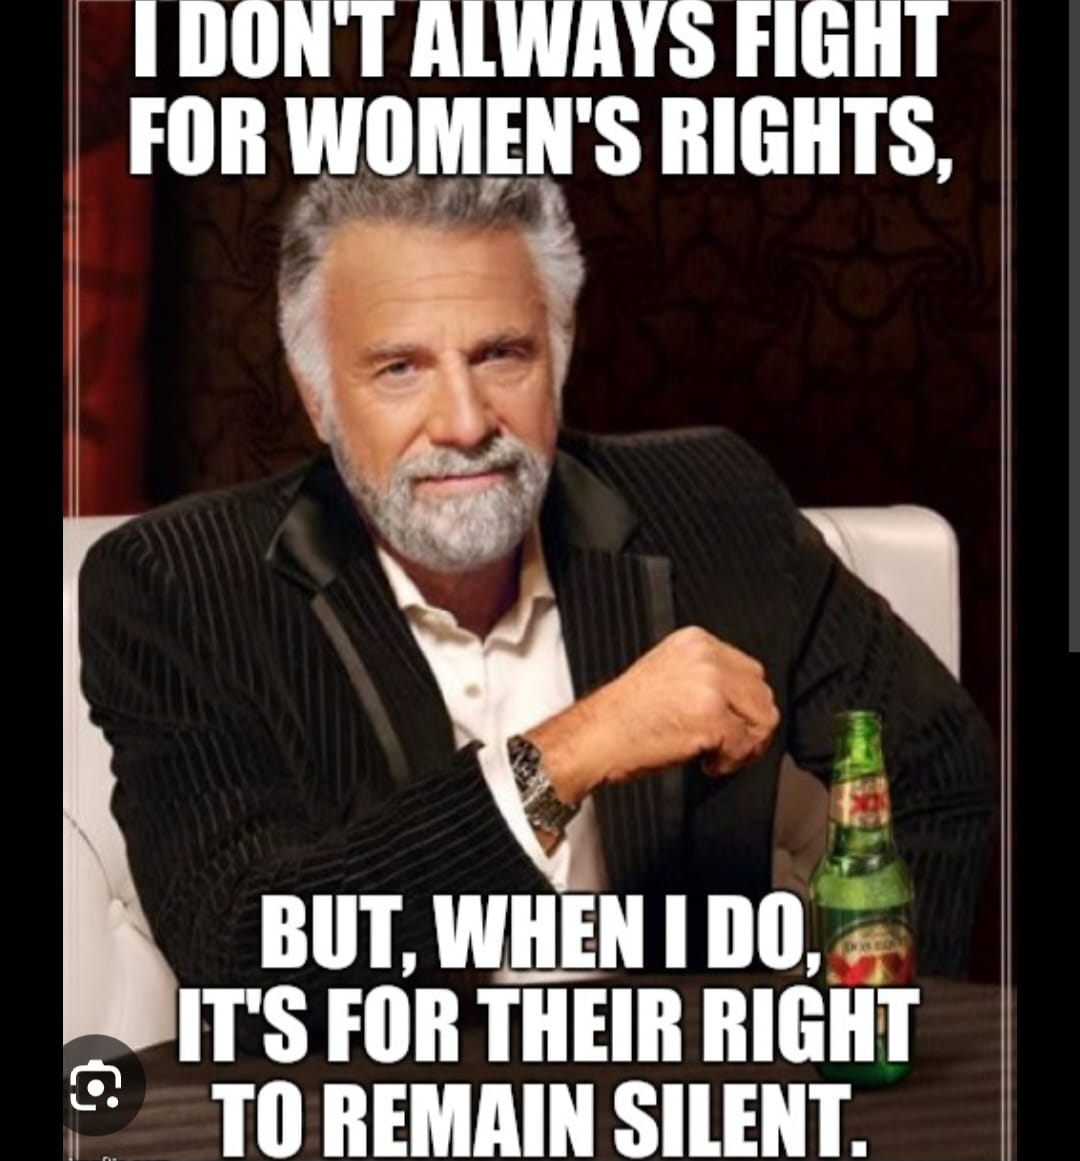
\includegraphics[
    width=0.078\textwidth,
    height=1.35cm,
    keepaspectratio
]{meme_respect_woman.jpeg}
&
women as a group
&
\makecell{\textit{Implicit-Harm}\\\textit{Misogyny}}
&
\makecell{\textit{Non-Harm}\\\textit{None}}
&
Conditional harm missed
&
The statement initially appears supportive of women but subsequently
conditions respect on satisfying unspecified gendered expectations.
The model overweights the positive phrase ``respect a woman.'' \\
\midrule

Q4 &

\includegraphics[
    width=0.078\textwidth,
    height=1.35cm,
    keepaspectratio
]{sports.jpeg}
&
women athletes
&
\makecell{\textit{Explicit-Harm}\\\textit{Misogyny}}
&
\makecell{\textit{Explicit-Harm}\\
\textit{Appearance-Attack}}
&
Category confusion
&
The model correctly detects explicit harm but misclassifies the
attack because it attends to the women shown in the image rather than
the textual denial of women's athletic ability and kitchen stereotype. \\
\midrule

Q5 &

\includegraphics[
    width=0.078\textwidth,
    height=1.35cm,
    keepaspectratio
]{popcorn.jpg}
&
woman speaker
&
\makecell{\textit{Non-Harm}\\\textit{None}}
&
\makecell{\textit{Explicit-Harm}\\
\textit{Sexual-Harassment}}
&
Lexical shortcut
&
The model over-relies on the phrase ``cop porn'' and predicts sexual
harm, although the meme presents a benign phonetic misunderstanding
without degrading or targeting the woman. \\
\midrule

Q6 &

\includegraphics[
    width=0.078\textwidth,
    height=1.35cm,
    keepaspectratio
]{weight.png}
&
wife
&
\makecell{\textit{Explicit-Harm}\\
\textit{Appearance-Attack}}
&
\makecell{\textit{Non-Harm}\\\textit{None}}
&
Humour masks harm
&
The conversational format obscures the appearance-based attack. The
model fails to recognize that the husband's response uses the wife's
weight as the basis of the joke. \\
\midrule

Q7 &

\includegraphics[
    width=0.078\textwidth,
    height=1.35cm,
    keepaspectratio
]{engine.jpg}
&
women as a group
&
\makecell{\textit{Implicit-Harm}\\\textit{Misogyny}}
&
\makecell{\textit{Non-Harm}\\\textit{None}}
&
Analogy-based stereotype missed
&
The meme compares women's anger to an unexplained warning light and
suggests that it should be ignored. The humorous analogy obscures the
stereotype that women's emotions are irrational and not worth
understanding. \\
\midrule

Q8 &

\includegraphics[
    width=0.078\textwidth,
    height=1.35cm,
    keepaspectratio
]{military.jpeg}
&
woman soldier
&
\makecell{\textit{Implicit-Harm}\\\textit{Misogyny}}
&
\makecell{\textit{Non-Harm}\\\textit{None}}
&
Contradictory framing
&
The empowering visual and statement about joining the military mask
the harmful implication that women invoke gender selectively to avoid
equal treatment. The model therefore mistakes the stereotype for
benign humour. \\
\bottomrule
\end{tabularx}

\caption{Qualitative error analysis on SheHarm-Meme. Gold and
predicted entries report harmfulness and harm category, respectively.
Errors arise from implicit stereotypes, competing categories,
conditional language, lexical shortcuts, humour, and image--text
interaction.}
\label{tab:qualitative_error_analysis}
\end{table*}



\end{document}
